
% ============================================================
% main_member2.tex — 成员2说明书
% 编译：xelatex main_member1.tex
% ============================================================

\documentclass{xautCADreport}

\title{冲压模具凸模与凹模数字化设计与制造课程设计}
\author{闫小杰}
\major{工业工程}
\class{工程232班}
\studentid{3230212007}
\advisor{董永亨\quad 侯晓莉}
\date{\today}

\begin{document}
\makecover
\renewcommand{\arraystretch}{1.3}

% --------------------------
% 中文摘要
% --------------------------
\begin{abstract}
本设计课题围绕冲压模具凸、凹模零件，开展了全流程数字化设计与制造的实践探索。通过使用SolidWorks软件\cite{ref:cad2020}完成零件的参数化建模与工程图绘制，精确表达了复杂的配合面及工艺特征；基于对零件加工难点与精度的深入分析，编制了详细的机械加工工艺规程，涵盖了从毛坯选择到精加工的全过程。随后，通过CAM技术生成刀具轨迹并导出NC代码，并借助\textbf{宇龙仿真\cite{ref:peng2020}软件}模拟实际机床切削环境，对加工程序进行了严格的干涉检查与轨迹优化；最终形成了一套高可靠性的数字化制造方案。通过本次设计，系统掌握了现代制造环境下模具零件“设计-工艺-仿真”的闭环开发模式，显著提升了工程实践素养。

\vspace{0.5em}

\noindent\zihao{-4}\heiti\bfseries 关键词：\zihao{-4}\songti 冲压模具；凹模；数字化建模；数控编程；宇龙仿真
\end{abstract}

\clearpage
\setcounter{tocdepth}{2}   % 目录只显示到二级标题（section和subsection）
\tableofcontents
\clearpage

\section{零件的数字化建模}

% ---- 1.1 零件的结构与工艺性分析 ----
\subsection{零件的结构与工艺性分析}

\subsubsection{零件的功能与用途}

本次课程设计的研究对象为冲压模具中的两大核心零件——凸模与凹模。该组零件属于板料冲裁模具的关键工作部件，其主要功能是在冲压设备驱动下，通过凸模与凹模之间的精确配合实现对金属板材的落料或冲孔加工。

\begin{figure}[htbp]
  \centering
  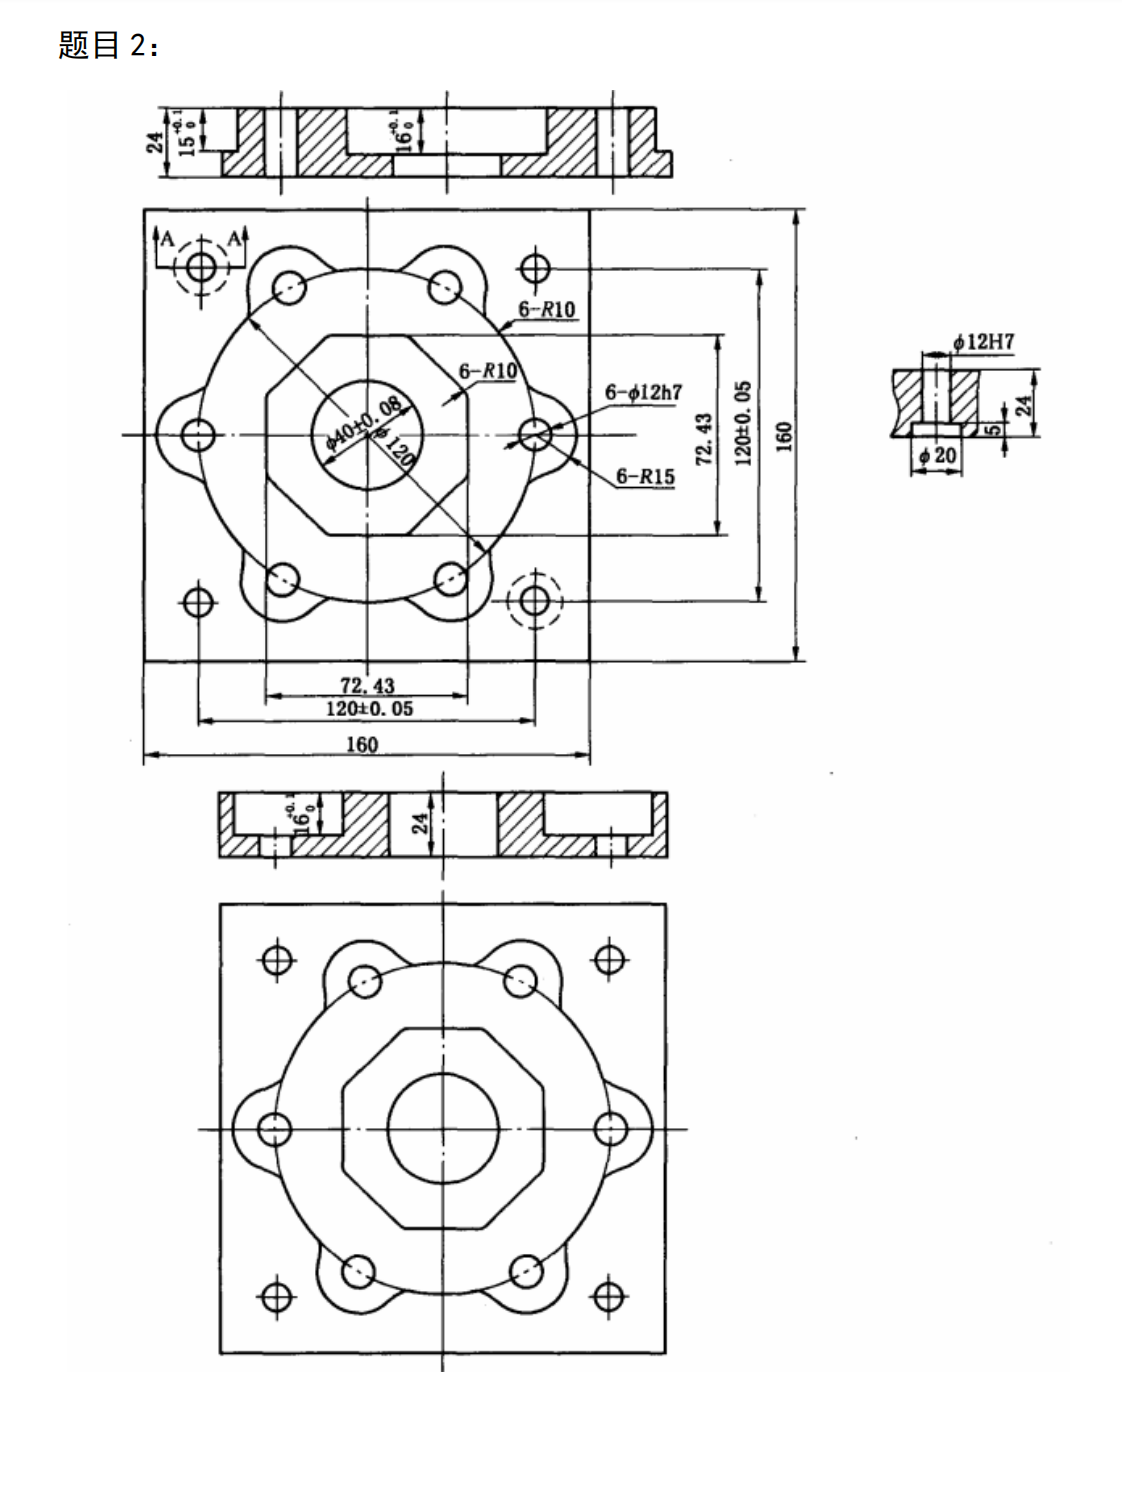
\includegraphics[width=0.75\textwidth]{figures/engineering_drawing.png}
  \caption{课程设计题目——凸模与凹模工程图}
  \label{fig:title_figure}
\end{figure}

\subsubsection{零件的结构特征}

\paragraph{（1）凹模的结构特征}

凹模整体呈方形板块结构，最大外形尺寸为$160\times160\times24\,\mathrm{mm}$。其主要结构要素包括：
\begin{enumerate}
  \item 中心型腔：八角形型腔，对边宽度$72.43\,\mathrm{mm}$，对角线长度$120\pm0.05\,\mathrm{mm}$；
  \item 螺钉过孔：共10个安装孔，其中6个$\phi12$孔位于中心花瓣槽处，4个$\phi10$孔位于四个角部；
  \item 减重工艺槽：6处花瓣状减重槽，由$R10$和$R15$圆弧组合而成。
\end{enumerate}

\paragraph{（2）凸模的结构特征}

凸模整体外形为$160\times160\times24\,\mathrm{mm}$方形板块，中央设有八角形凸台结构，与凹模型腔形成间隙配合关系，并加工有10个安装通孔。

\subsubsection{材料选用与热处理要求}

选用45钢作为两零件的材料。粗加工后进行调质处理（840℃水冷淬火+580℃高温回火），硬度控制在HB220～250；精加工后工作表面采用表面淬火处理，硬度达到HRC48～52。

% ---- 1.2 零件的三维建模 ----
\subsection{零件的三维建模}

本节使用SolidWorks软件对凸模和凹模进行参数化三维实体建模。建模过程遵循"先主体后细节、先外廓后内腔"的基本原则，通过拉伸凸台、拉伸切除、异形孔向导等特征操作逐步构建零件的完整几何模型。

\subsubsection{凹模的建模过程}

凹模的整体建模思路为：首先创建方形基体，然后依次去除型腔、孔系及减重槽等内部特征。具体建模步骤如下：

\paragraph{（1）创建方形基体}

在"上视基准面"上绘制$160\times160\,\mathrm{mm}$的正方形草图，利用"拉伸凸台"命令沿法向拉伸$24\,\mathrm{mm}$，生成凹模的方形板块基体。基体为后续所有切除特征提供了依附的几何载体。

\paragraph{（2）切除八角形型腔及中心孔}

在基体上表面绘制八角形型腔草图。八角形对边宽度为$72.43\,\mathrm{mm}$，对角线长度$120\,\mathrm{mm}$，8个顶点均匀分布于以$60\pm0.025\,\mathrm{mm}$为外接圆半径的圆周上。利用"拉伸切除"命令向下贯穿基体，切除深度为$24\,\mathrm{mm}$（贯通）。型腔中央设有$\phi40\,\mathrm{mm}$通孔，采用"拉伸切除"命令从上表面贯穿至下表面。

\paragraph{（3）切除6个花瓣状减重槽}

凹模上均布6处花瓣状减重槽，由$R10$和$R15$两组圆弧交替连接而成，均匀分布于八角形型腔与外形之间。在基体上表面绘制花瓣槽轮廓草图，利用"拉伸切除"命令向下贯穿基体。6处槽型通过"圆周阵列"命令（阵列数6、$360^{\circ}$均布）快速完成。

\paragraph{（4）创建6个$\phi12\,\mathrm{H7}$通孔及沉孔}

利用SolidWorks的"异形孔向导"功能，选择"直螺纹孔"类型，孔径$\phi12\,\mathrm{mm}$，精度等级H7，贯穿方式为"完全贯穿"。6个孔以八角形中心为基准，均布于$\phi110\,\mathrm{mm}$的圆周上（通过"圆周阵列"命令实现）。每个孔上部设有$\phi20\,\mathrm{mm}$、深$5\,\mathrm{mm}$的沉头孔，同样通过"异形孔向导"中的沉头孔选项完成。

\begin{figure}[H]
  \centering
  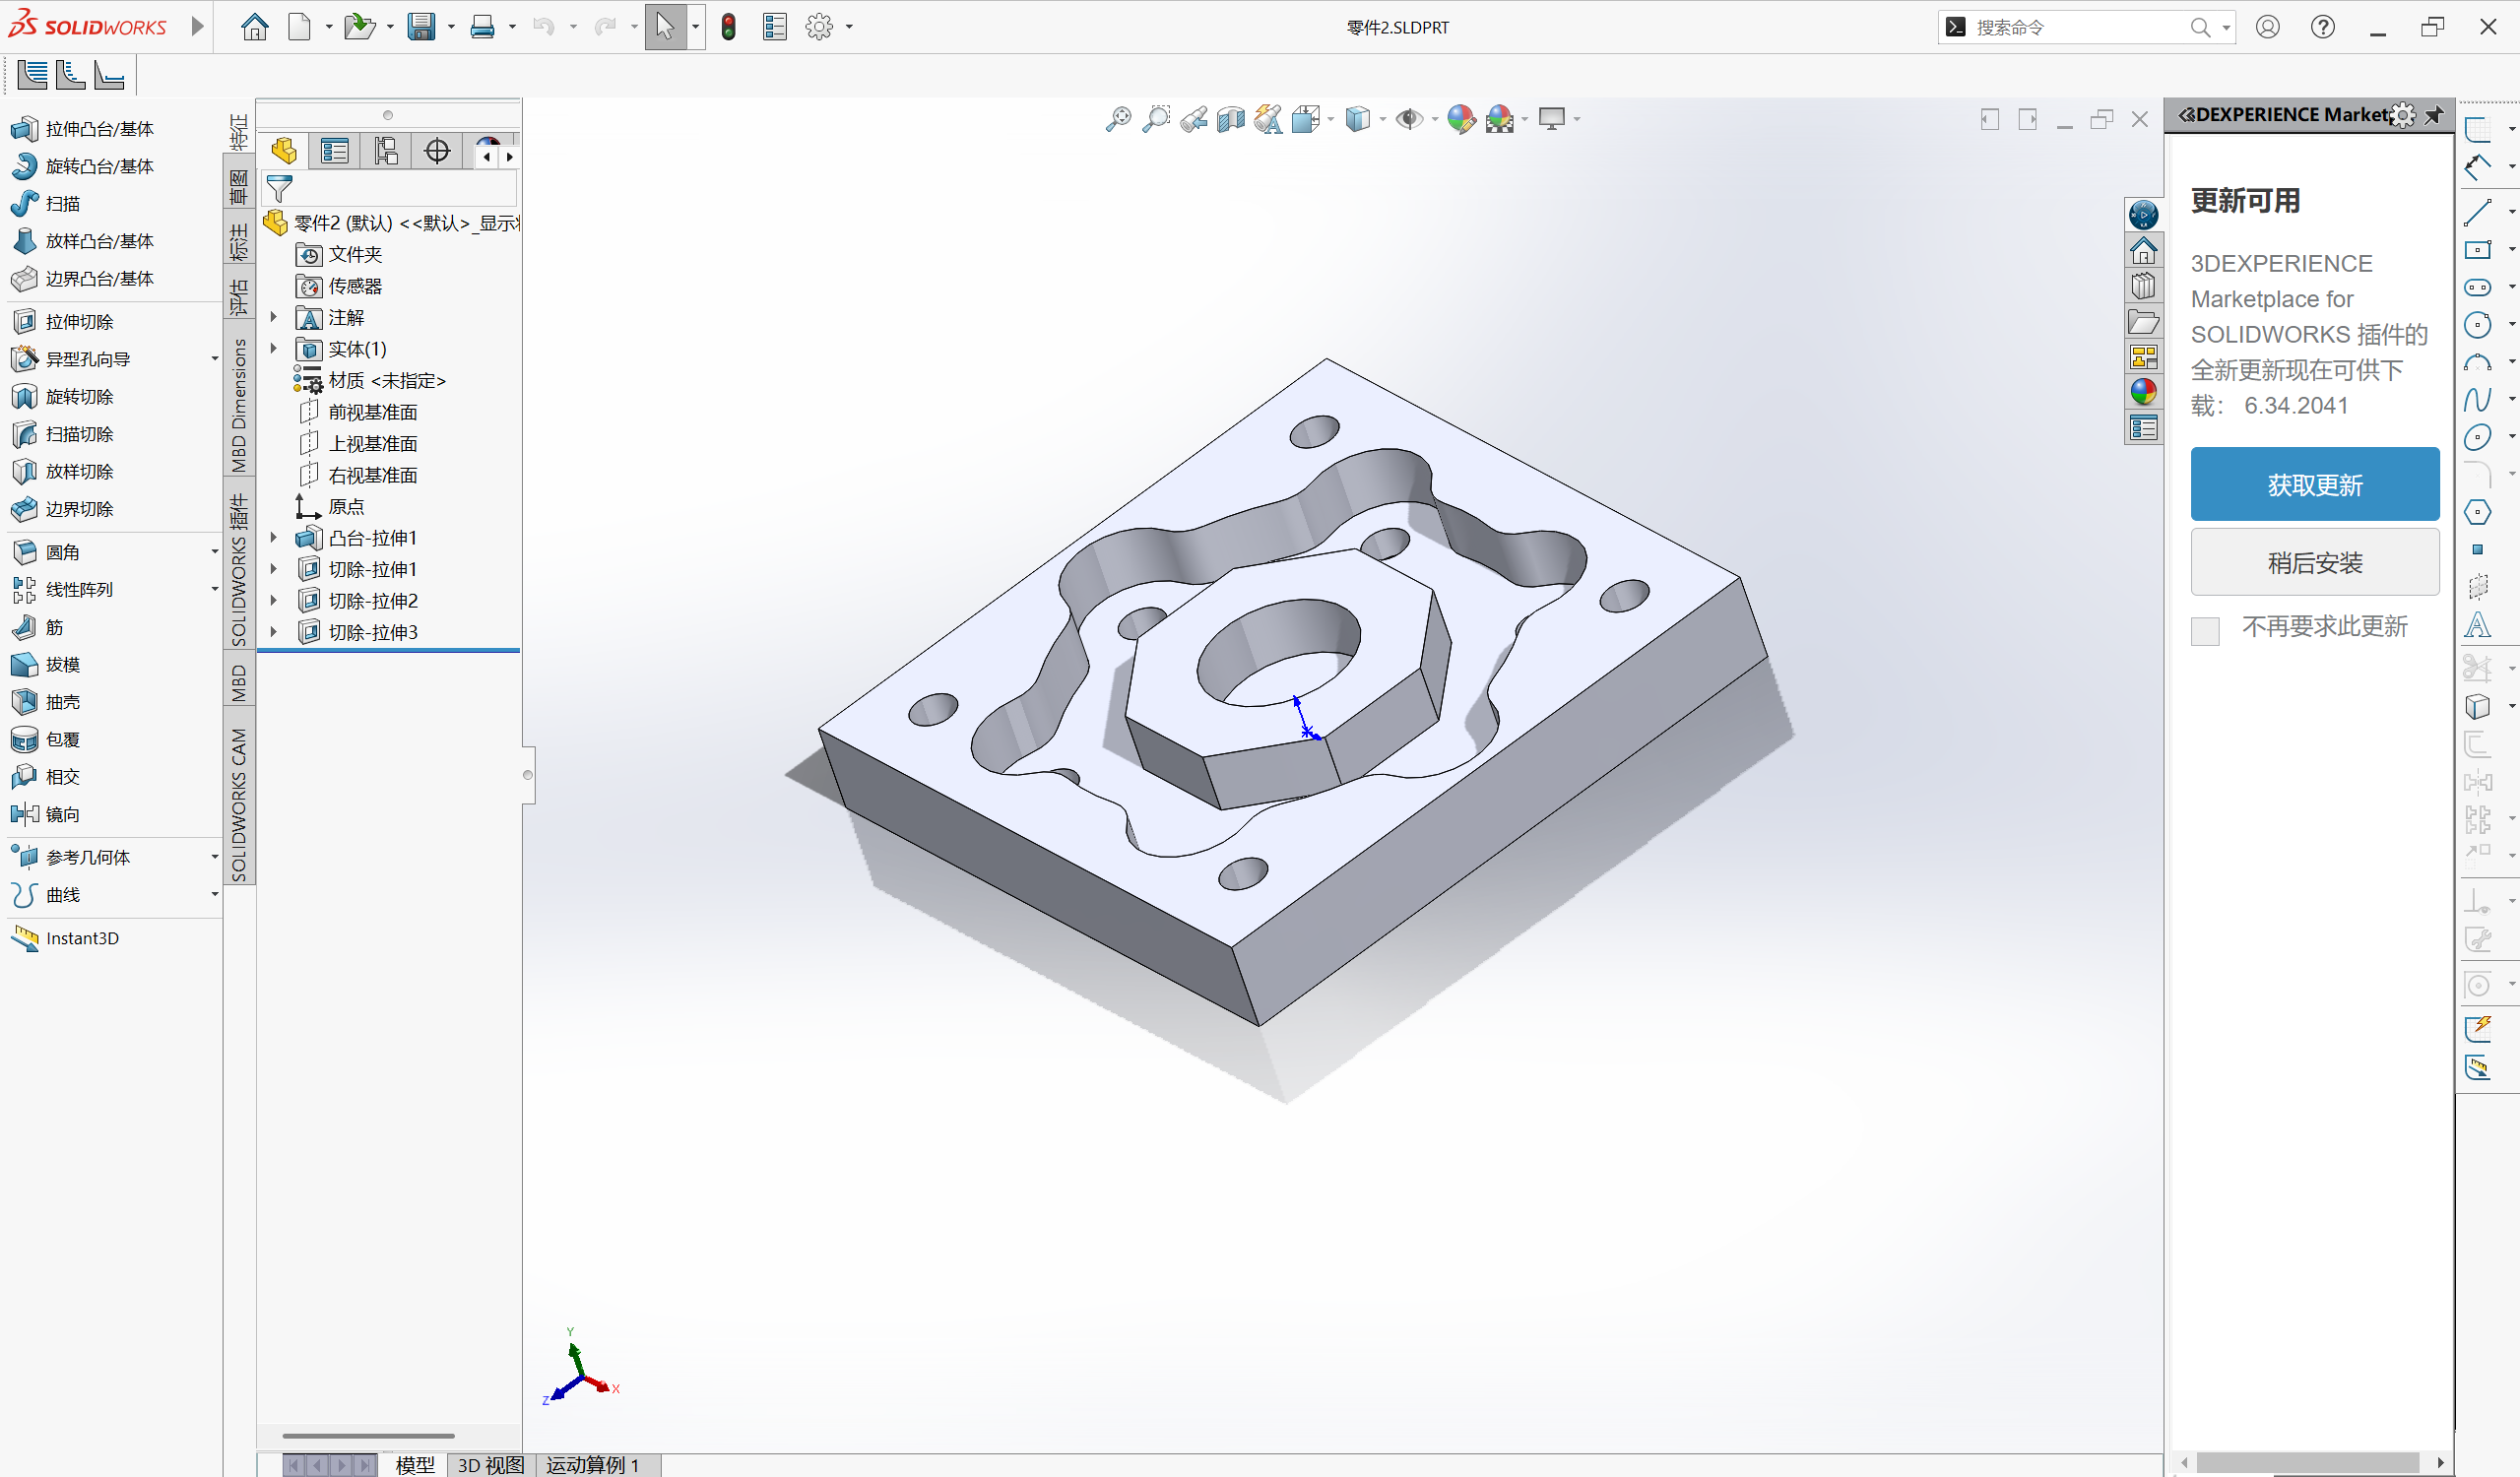
\includegraphics[width=0.75\textwidth]{figures/凹模三维图.png}
  \caption{凹模三维实体模型}
  \label{fig:die_3d}
\end{figure}

\subsubsection{凸模的建模过程}

凸模的整体外形与凹模相同（$160\times160\times24\,\mathrm{mm}$方形板块），核心区别在于中心特征为"拉伸凸台"形成的八角形凸台而非切除型腔。具体建模步骤如下：

\paragraph{（1）创建方形基体}

与凹模完全相同，在"上视基准面"绘制$160\times160\,\mathrm{mm}$正方形草图，拉伸$24\,\mathrm{mm}$生成板块基体。

\paragraph{（2）创建八角形凸台}

在基体上表面绘制八角形凸台草图，对边宽度$72.43\,\mathrm{mm}$，对角线$120\,\mathrm{mm}$。利用"拉伸凸台"命令向上拉伸$16\,\mathrm{mm}$，形成与凹模型腔配合的八角形凸台结构。凸台中心设有$\phi40\,\mathrm{mm}$通孔，采用"拉伸切除"命令从凸台顶面贯穿至基体底面。

\paragraph{（3）切除6个花瓣状减重槽}

凸模的花瓣槽结构与凹模相同，均为$R10$与$R15$圆弧组合，均布于八角形凸台与外形之间。建模方法与凹模一致：绘制草图后"拉伸切除"贯穿基体，再通过"圆周阵列"复制6组。

\paragraph{（4）创建10个安装通孔及沉孔}

孔系的规格、分布（10个孔包含6个12孔和4个10孔）与位置与凹模保持一致，建模方法相同。

\begin{figure}[H]
  \centering
  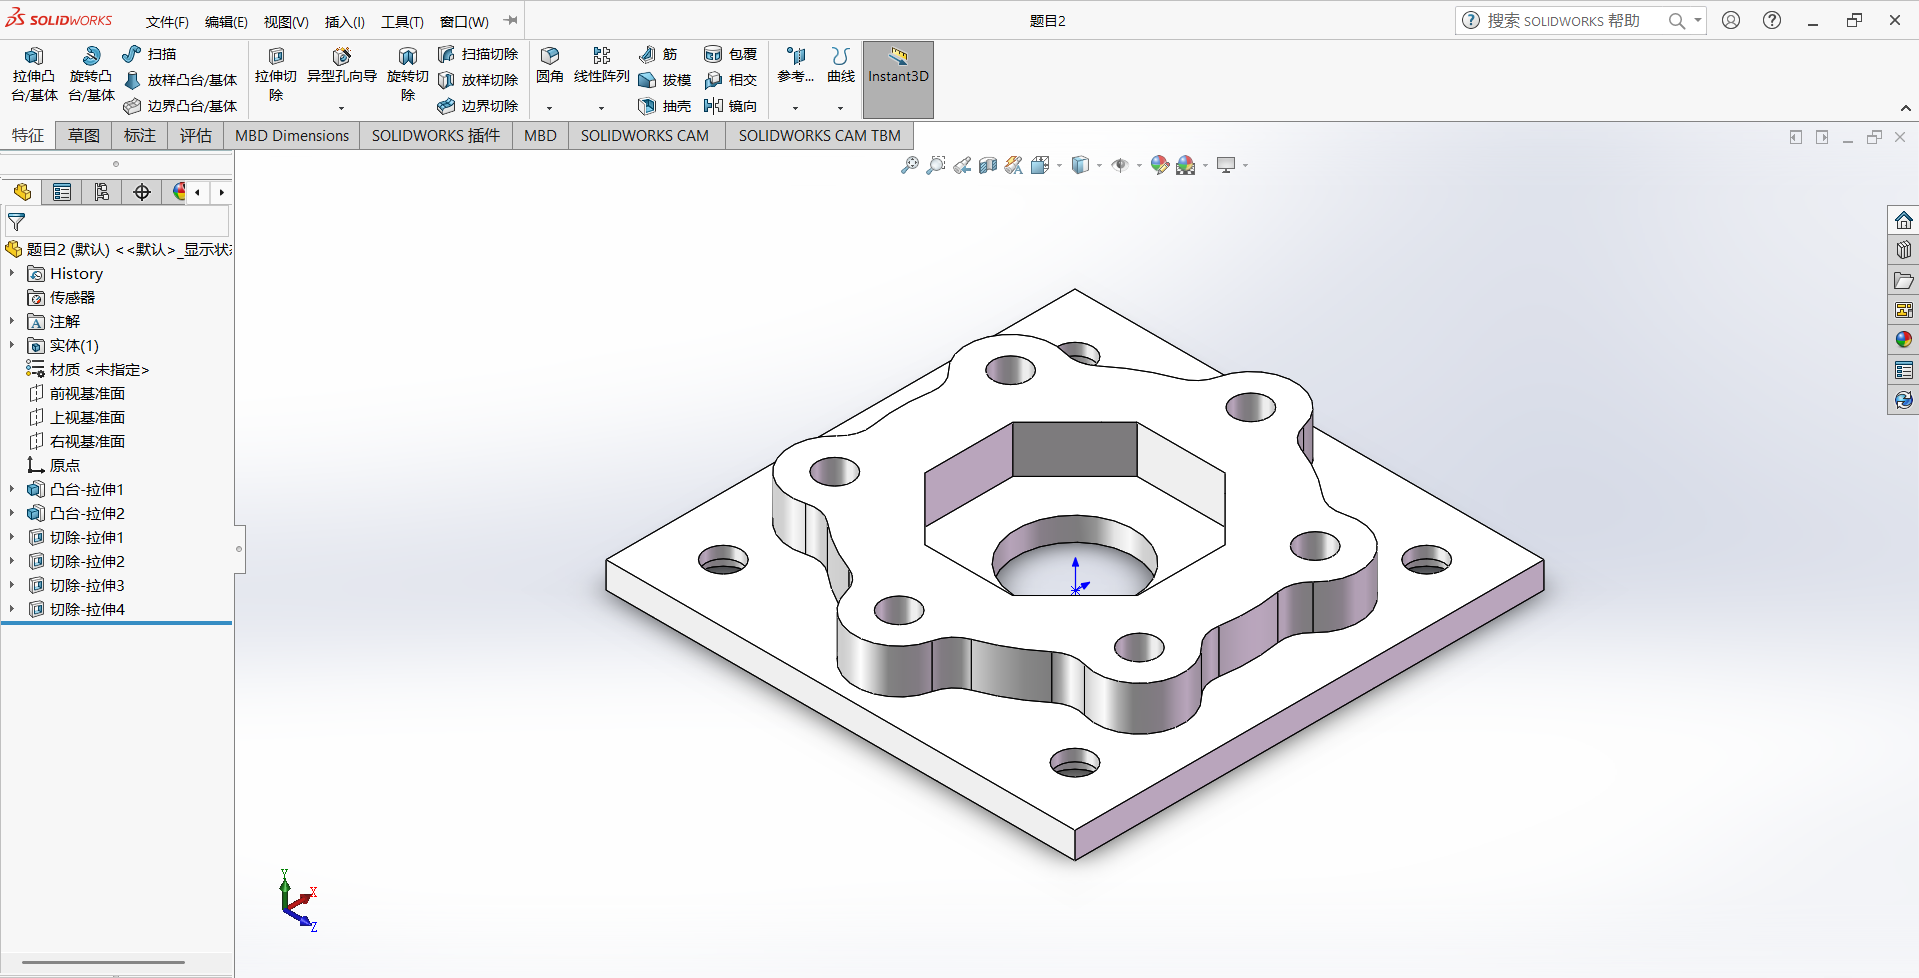
\includegraphics[width=0.75\textwidth]{figures/凸模三维图.png}
  \caption{凸模三维实体模型}
  \label{fig:punch_3d}
\end{figure}

\subsubsection{建模过程对比}

凹模与凸模的建模过程对比如表\ref{tab:modeling_compare}所示。

\begin{table}[H]
  \centering
  \caption{凹模与凸模建模过程对比}
  \label{tab:modeling_compare}
  \begin{tabular}{lll}
    \toprule
    建模步骤 & 凹模 & 凸模 \\
    \midrule
    基体创建 & 拉伸凸台$160\times160\times24$ & 拉伸凸台$160\times160\times24$ \\
    中心特征 & 拉伸切除（八角形型腔） & 拉伸凸台（八角形凸台） \\
    花瓣槽 & 拉伸切除 + 圆周阵列 & 拉伸切除 + 圆周阵列 \\
    孔系 & 异形孔向导 + 圆周阵列 & 异形孔向导 + 圆周阵列 \\
    \bottomrule
  \end{tabular}
\end{table}

% ---- 1.3 零件工程图的绘制 ----
\subsection{零件工程图的绘制}

三维模型完成后，需将其转化为符合国家标准的二维工程图，用于指导实际生产加工。本节详细阐述凸模和凹模工程图的绘制过程与标注要求。

\subsubsection{工程图绘制的基本原则}

工程图绘制遵循以下原则：
\begin{enumerate}
  \item 图纸幅面与格式：选用GB/T 14689—2008规定的A3幅面（$420\,\mathrm{mm}\times297\,\mathrm{mm}$），横放布置，留有装订边；
  \item 比例选择：根据零件尺寸大小选用适当比例，采用1:2缩小比例；
  \item 投影法：采用第一角投影法，符合GB/T 14692—2008的规定；
  \item 尺寸标注：遵循GB/T 4458.4—2003《机械制图 尺寸注法》的规范要求。
\end{enumerate}

\subsubsection{视图方案设计}

根据凸模和凹模的结构特点，确定如下视图方案：

\begin{itemize}
  \item 主视图：采用俯视方向投影，完整表达零件的外廓形状、八角形轮廓（凸台/型腔）、孔系及花瓣槽的分布情况；
  \item 全剖视图：沿零件对称面剖切，清晰展示八角形型腔（凹模）或凸台（凸模）的深度、$\phi40$中心孔的贯穿情况以及$24\,\mathrm{mm}$的总厚度；
\end{itemize}

\subsubsection{尺寸与公差标注}

工程图中的尺寸标注遵循"功能尺寸直接标注、非功能尺寸按加工顺序标注"的原则，主要包括：

\paragraph{（1）凹模的尺寸标注}

\begin{enumerate}
  \item 外形尺寸：总长$160\,\mathrm{mm}$、总宽$160\,\mathrm{mm}$、总厚$24\,\mathrm{mm}$，外形公差按GB/T 1804—m级（中等精度）未注公差控制；
  \item 八角形型腔尺寸：对角线长度$120\pm0.05\,\mathrm{mm}$（关键配合尺寸，直接影响冲裁间隙均匀性），对边宽度$72.43\,\mathrm{mm}$，型腔外外接圆半径$R60\pm0.025\,\mathrm{mm}$；
  \item 中心孔尺寸：$\phi40\,\mathrm{mm}$通孔，配合精度H7；
  \item 孔系尺寸：共10个安装孔，其中6个$\phi12\,\mathrm{H7}$孔（均布于中心圆周）和4个$\phi10\,\mathrm{mm}$孔（均布于角部），上表面均设有$\phi20\times5\,\mathrm{mm}$受沉头孔；
  \item 花瓣槽尺寸：6处花瓣状减重槽，由$R10$和$R15$两组圆弧交替连接，均布于型腔与外形之间；
  \item 形位公差：上下两大平面的平行度公差$0.02\,\mathrm{mm}$，侧面对底面的垂直度公差$0.03\,\mathrm{mm}$，八角形型腔相对于$\phi40$中心孔的同轴度公差$\phi0.03\,\mathrm{mm}$。
\end{enumerate}

\paragraph{（2）凸模的尺寸标注}

\begin{enumerate}
  \item 外形尺寸：总长$160\,\mathrm{mm}$、总宽$160\,\mathrm{mm}$、总厚$24\,\mathrm{mm}$，与凹模一致；
  \item 八角形凸台尺寸：对角线长度$120\,\mathrm{mm}$，对边宽度$72.43\,\mathrm{mm}$，凸台高度$16\,\mathrm{mm}$，与凹模型腔形成间隙配合；
  \item 中心孔尺寸：$\phi40\,\mathrm{mm}$通孔，贯穿凸台与基体；
  \item 孔系尺寸：10个安装孔（6个$\phi12$和4个$\phi10$），均布于对应定位坐标，沉孔$\phi20\times5\,\mathrm{mm}$，与凹模完全对应；
  \item 花瓣槽尺寸：结构与凹模相同，$R10$与$R15$圆弧组合，6处均布；
  \item 形位公差：上下平面平行度$0.02\,\mathrm{mm}$，凸台侧面与底面垂直度$0.03\,\mathrm{mm}$，凸台与中心孔同轴度$\phi0.03\,\mathrm{mm}$。
\end{enumerate}

上述尺寸中，八角形对角线尺寸$120\pm0.05\,\mathrm{mm}$为最重要的配合尺寸，其公差带大小仅$0.10\,\mathrm{mm}$，需通过精铣工序严格保证。安装孔系的精度等级均要求较高，需采用钻→扩→铰的加工方案方能达到。

\subsubsection{表面粗糙度标注}

根据各加工表面的功能要求，标注相应的表面粗糙度值：
\begin{itemize}
  \item 上下两大平面：$Ra1.6\,\mu\mathrm{m}$（基准面，需精铣或磨削保证，影响零件装配精度与配合质量）；
  \item 八角形配合面（凹模型腔内壁/凸模凸台外壁）：$Ra1.6\,\mu\mathrm{m}$（关键配合面，直接影响冲裁间隙与冲压件质量）；
  \item $\phi10/\phi12$孔内表面：$Ra1.6\,\mu\mathrm{m}$（精密定位孔，需铰孔保证，配合精度IT7）；
  \item $\phi40$中心孔内表面：$Ra3.2\,\mu\mathrm{m}$（一般配合孔，精镗即可满足）；
  \item 花瓣槽底面及侧面：$Ra3.2\,\mu\mathrm{m}$（非关键配合面，数控铣削一次精加工保证）；
  \item 四周侧面：$Ra3.2\,\mu\mathrm{m}$（非配合面，数控铣削保证）；
  \item 其余非配合表面：$Ra6.3\,\mu\mathrm{m}$（粗加工面或非加工面，不做特殊要求）。
\end{itemize}

上述表面粗糙度要求中，$Ra1.6\,\mu\mathrm{m}$等级的表面共包括两大平面、八角形配合面和10个定位孔内壁，是本零件加工中需重点保证的关键表面。在工艺路线制定时，需安排精铣或磨削工序以满足其粗糙度要求。

从上述表面粗糙度要求的分布可以看出，零件的关键表面主要集中在$Ra1.6\,\mu\mathrm{m}$等级。根据金属切削加工的一般规律，铣削加工通常可以达到$Ra3.2\sim Ra1.6\,\mu\mathrm{m}$的表面质量，而磨削加工则可以将表面质量进一步提升至$Ra0.8\sim Ra0.4\,\mu\mathrm{m}$。鉴于本次课程设计采用三轴数控铣床作为主要加工设备，对于上下两大平面，在精铣之后安排一道平面精磨工序，以确保$Ra1.6\,\mu\mathrm{m}$的最终表面粗糙度和上下平面之间的$0.02\,\mathrm{mm}$平行度要求。对于八角形配合面（凹模型腔内壁和凸模凸台外壁），由于其为侧向曲面且难以磨削加工，需依靠高精度数控精铣配合小切深、低进给的切削策略，力争在铣削阶段直接达到$Ra1.6\,\mu\mathrm{m}$的粗糙度指标。对于10个精密定位孔，采用钻$\to$扩$\to$铰的三段式加工方案，其中铰孔工序可将孔壁粗糙度提升至$Ra1.6\sim Ra0.8\,\mu\mathrm{m}$，完全满足IT7级精度和粗糙度要求。由此可见，表面粗糙度的工艺保证是贯穿整个工艺路线设计的重要约束条件，须在每一道工序的刀具选型、切削参数选择和走刀策略中予以具体落实。



\begin{figure}[H]
  \centering
  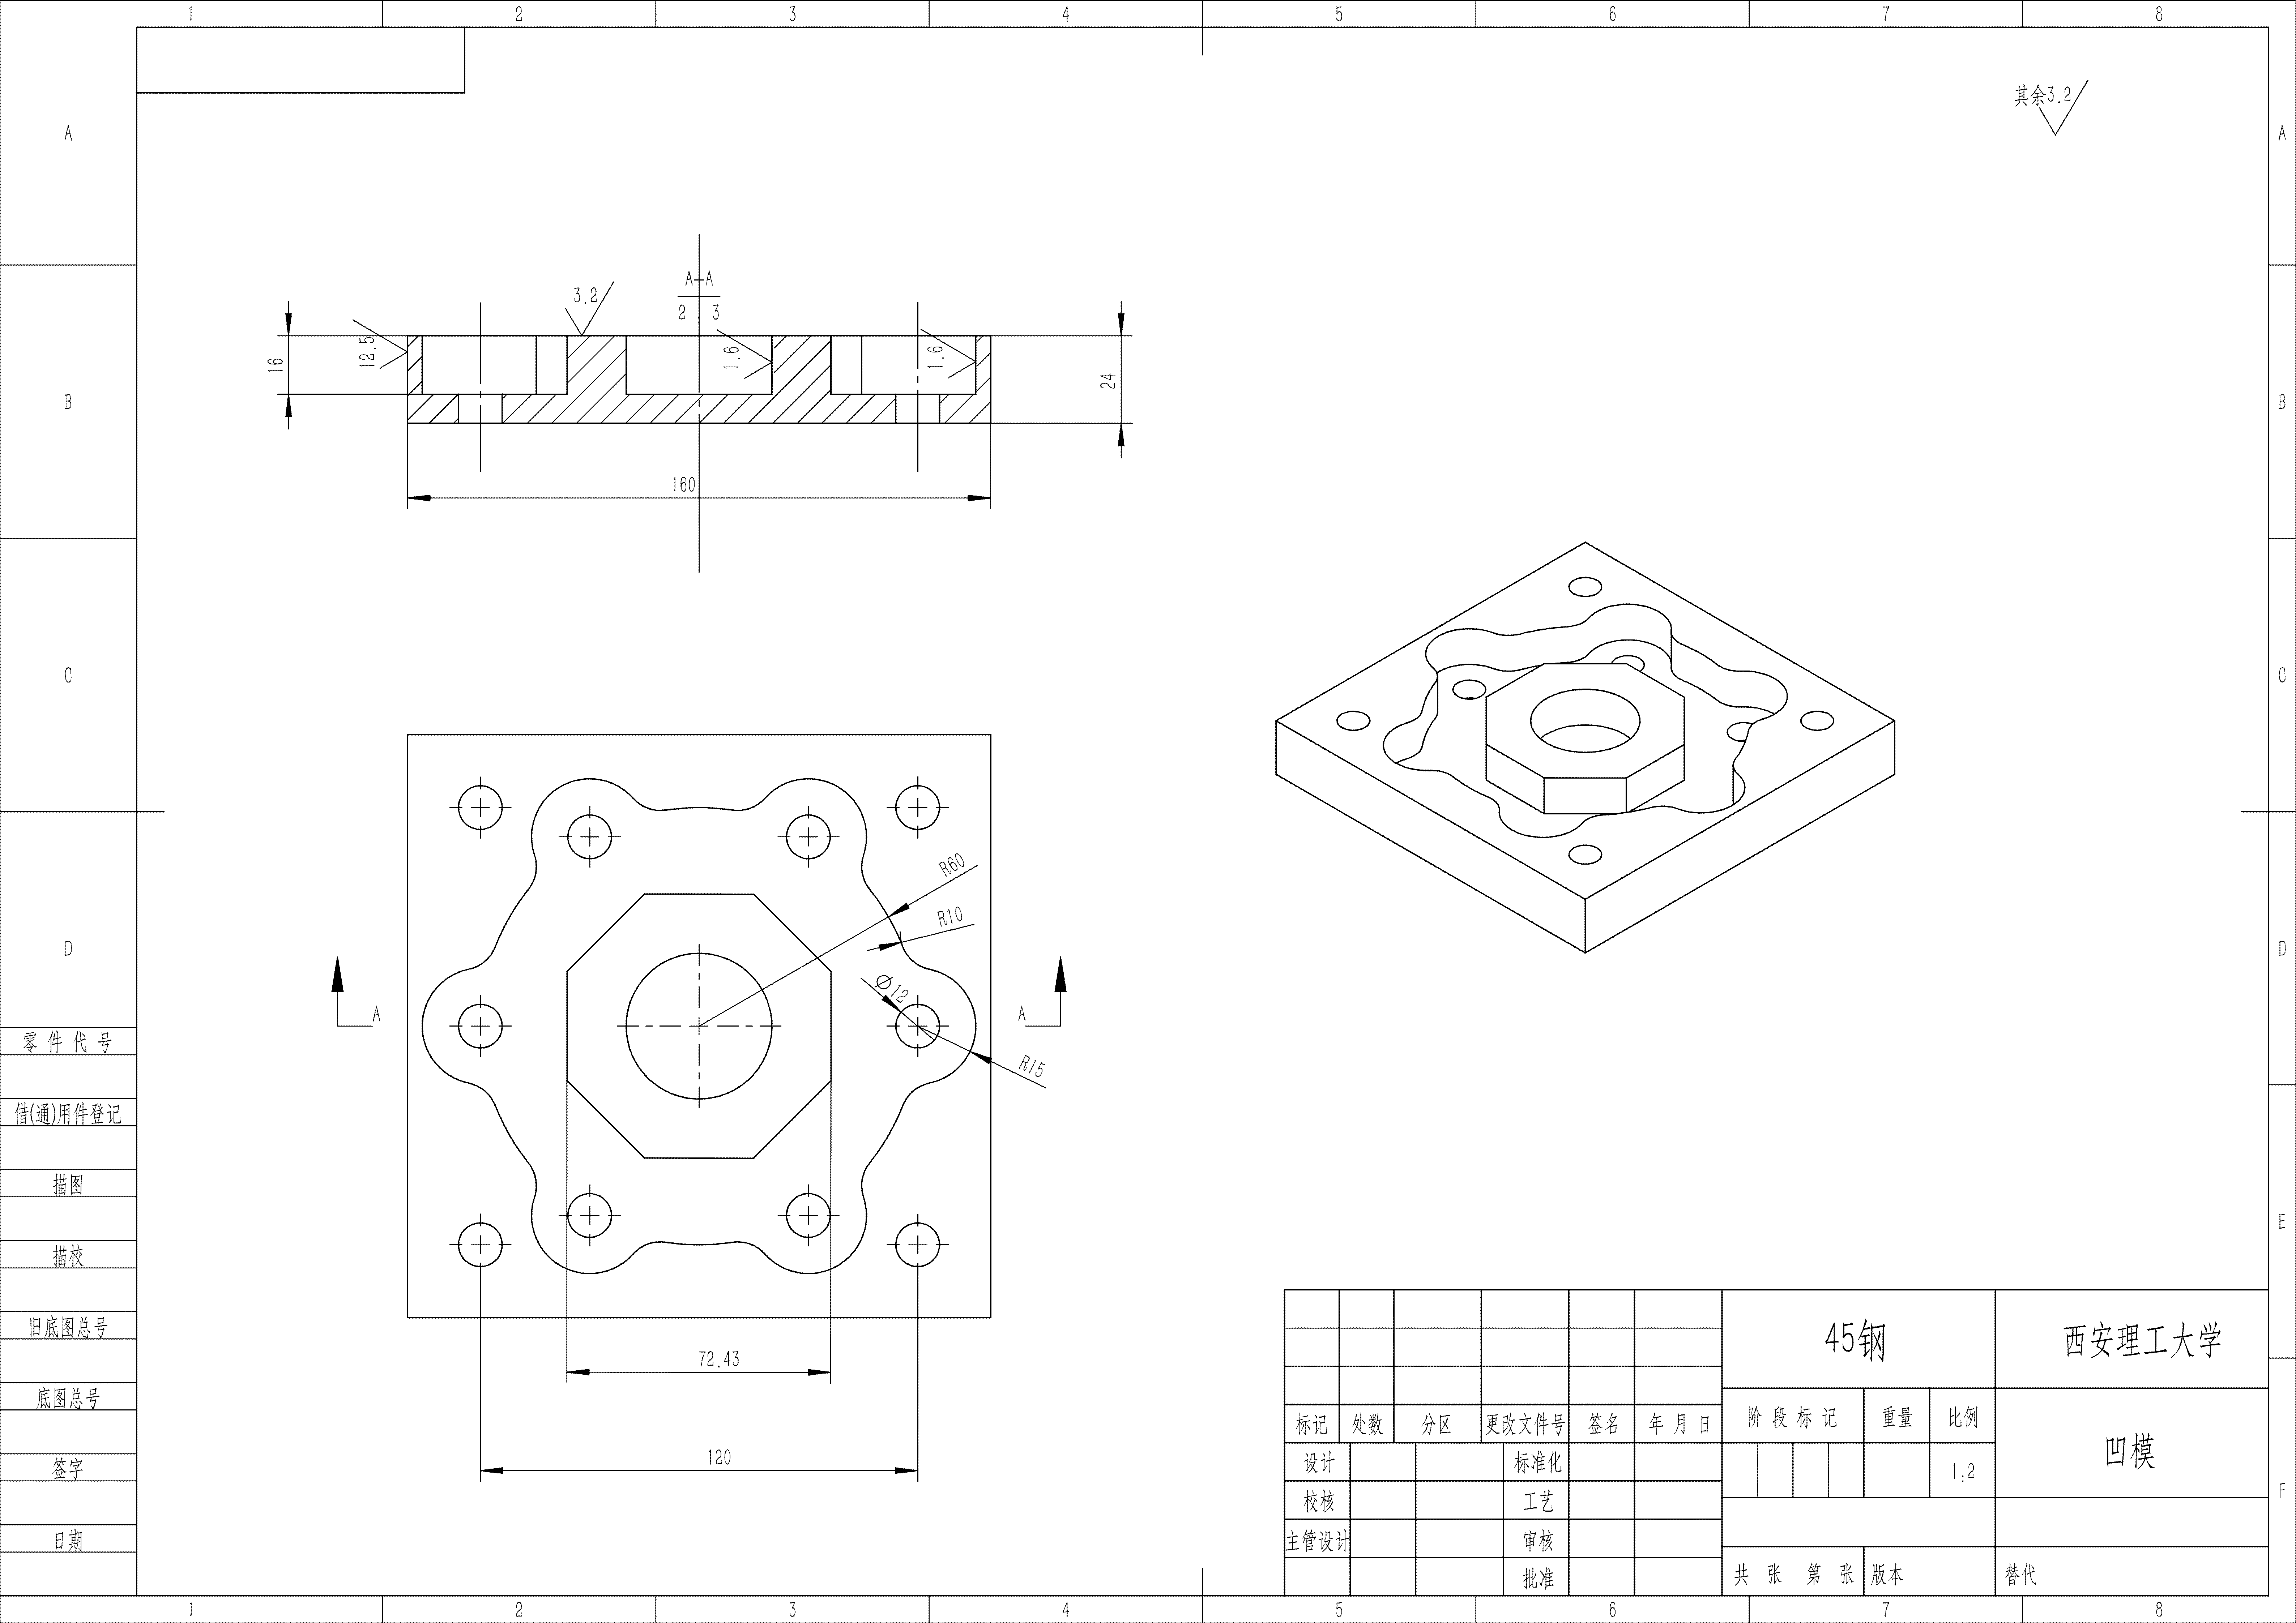
\includegraphics[width=0.9\textwidth]{figures/drawing_die_p1.png}
  \caption{凹模工程图}
  \label{fig:die_drawing}
\end{figure}

\begin{figure}[H]
  \centering
  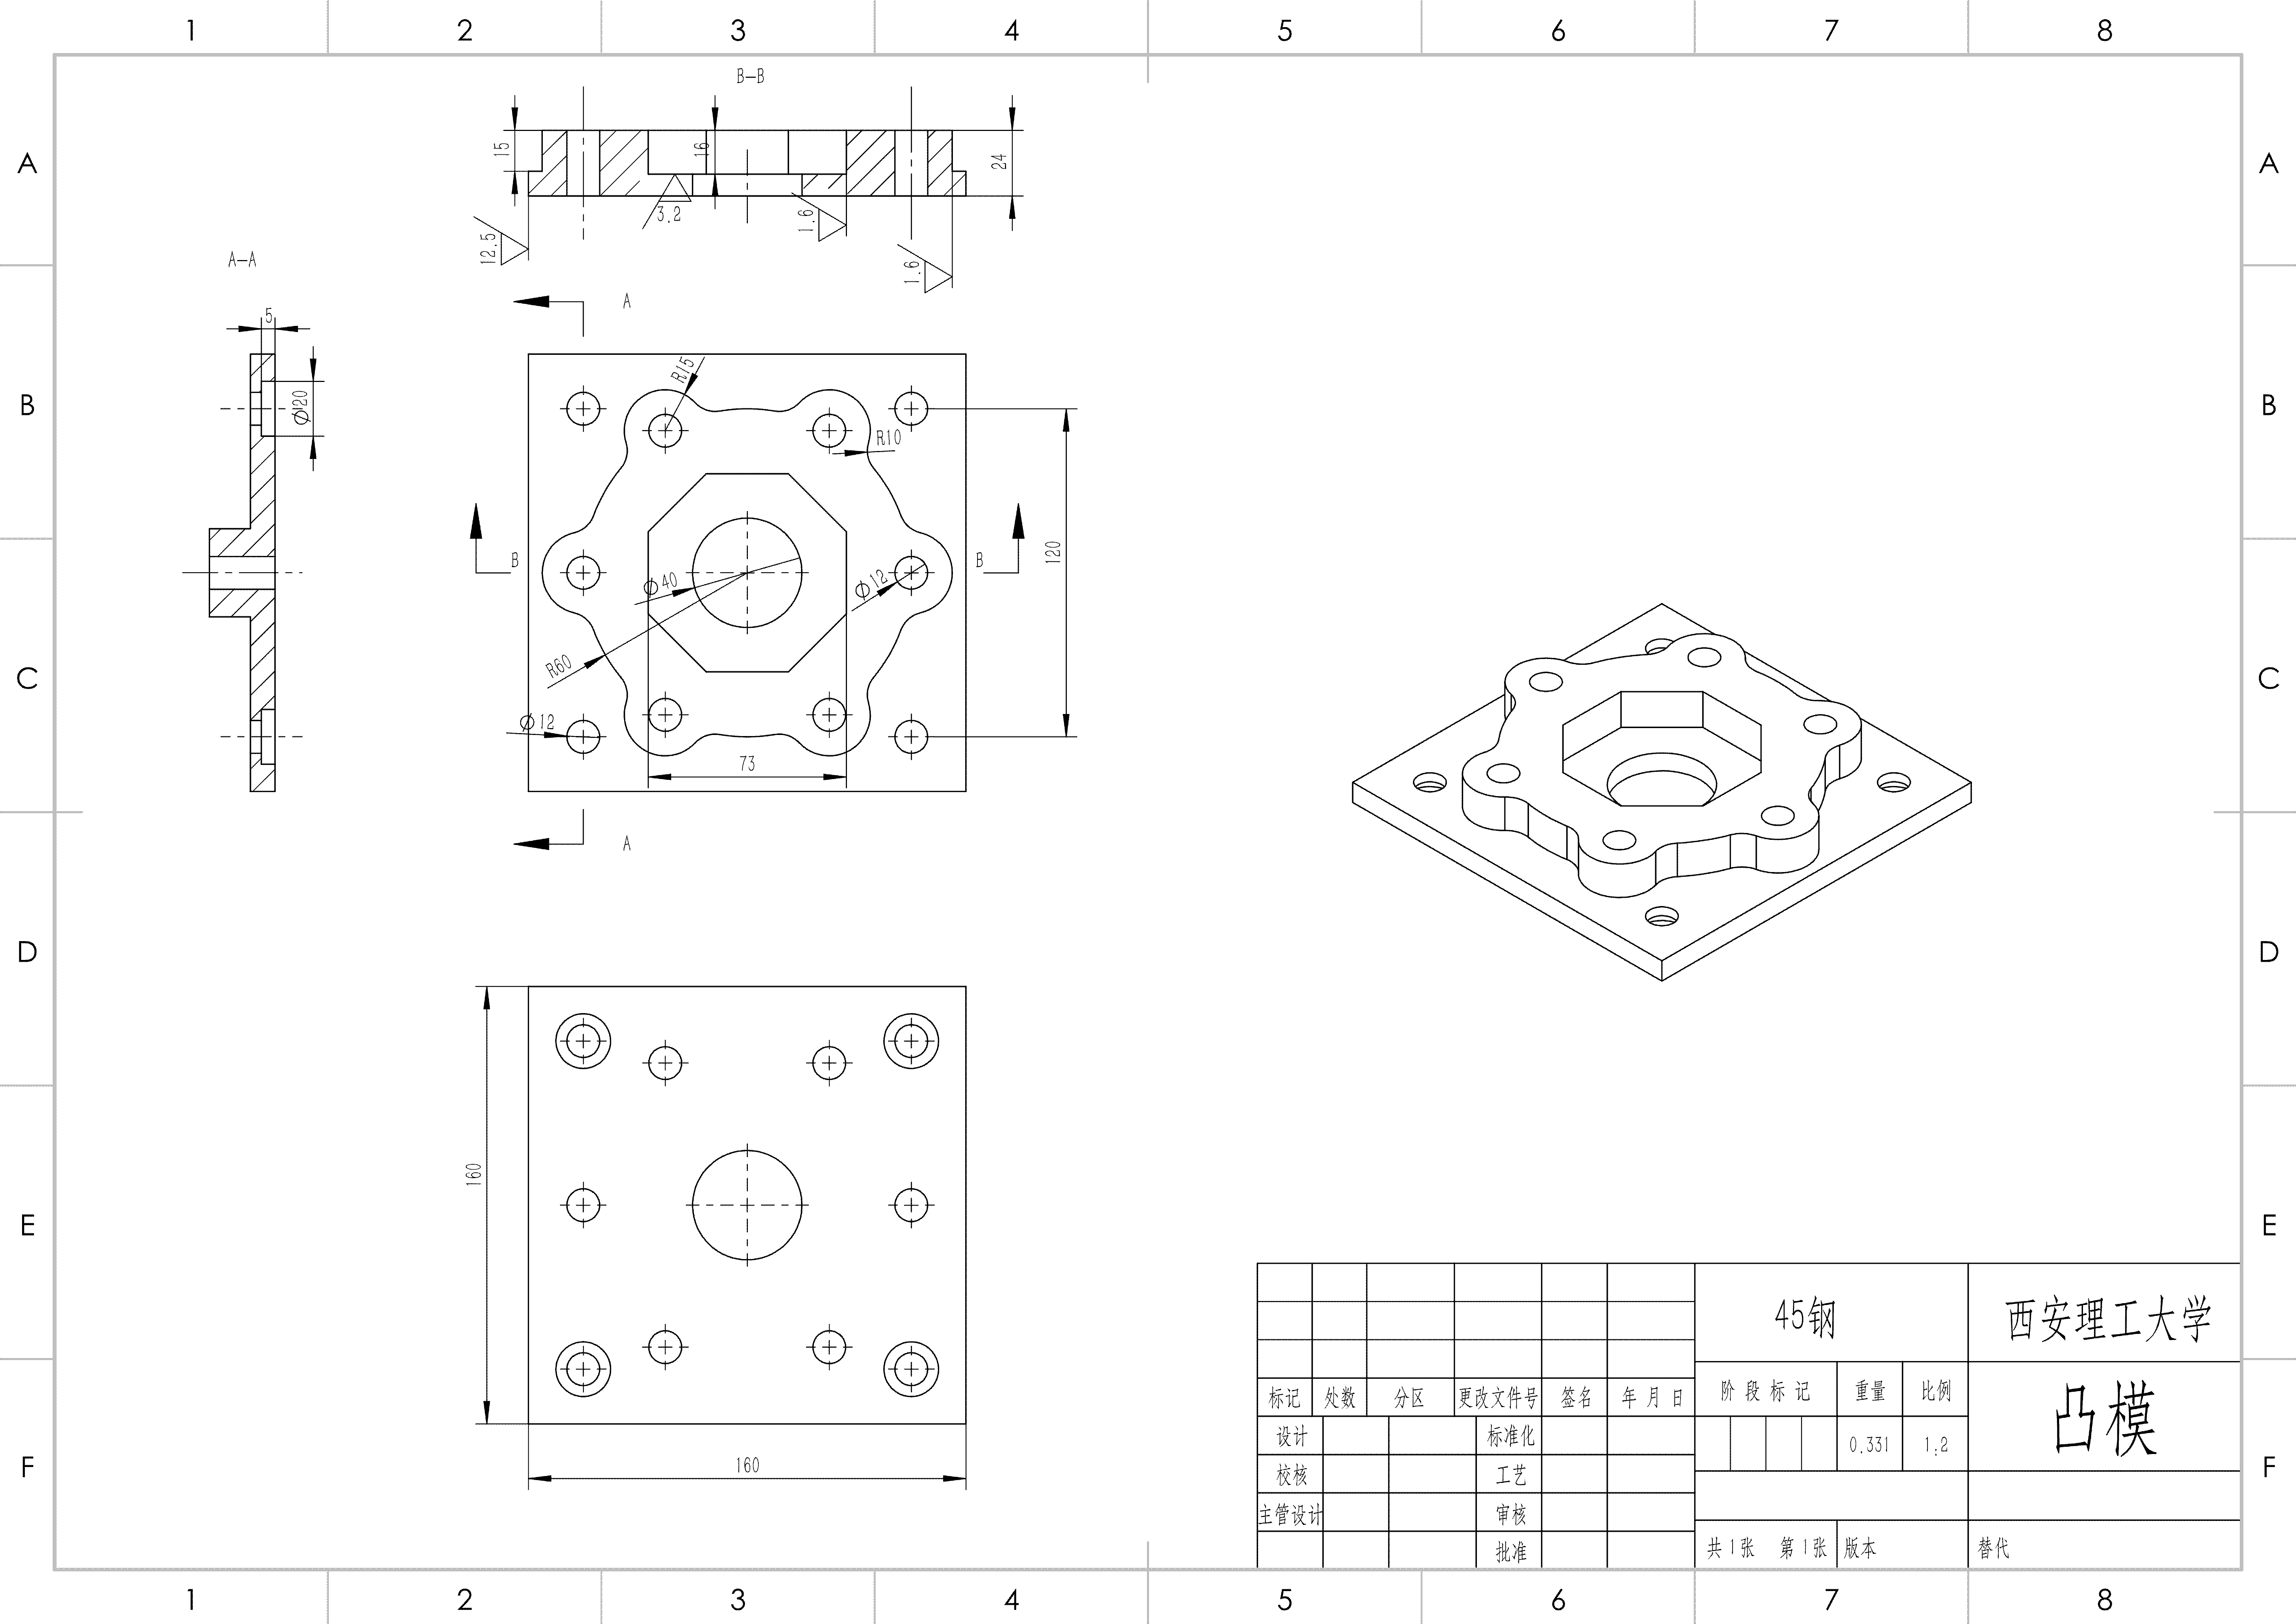
\includegraphics[width=0.9\textwidth]{figures/drawing_punch_p1.png}
  \caption{凸模工程图}
  \label{fig:punch_drawing}
\end{figure}

\clearpage
% ============================================================
% 第二章 加工工艺分析及编程
% ============================================================

\newpage

\section{加工工艺分析及编程}

% ---- 2.1 零件加工工艺性分析 ----
\subsection{零件加工工艺性分析}

\subsubsection{凸模加工工艺性分析}

凸模的整体结构为$160\times160\times24\,\mathrm{mm}$方形板块，中央设有八角形凸台，凸台高度$16\,\mathrm{mm}$，对角线尺寸$120\pm0.05\,\mathrm{mm}$。零件材料为45钢，经调质处理后硬度达220~255HBW，切削加工性良好。从工艺角度分析，凸模加工具有以下特点：

\begin{enumerate}
  \item 结构对称性好：零件整体呈中心对称结构，八角形凸台、10个安装孔及6处花瓣槽均以中心对称分布，适合采用数控铣削的圆周阵列功能进行加工；
  \item 刚性适中：零件厚宽比为$24/160=0.15$，属于板块类零件，装夹时需注意防止夹紧变形；
  \item 关键配合面精度要求高：八角形凸台侧面的尺寸公差$120\pm0.05\,\mathrm{mm}$、表面粗糙度$Ra1.6\,\mu\mathrm{m}$以及与底面的垂直度$0.03\,\mathrm{mm}$均需精铣或磨削工序保证；
  \item 孔系精度要求：10个安装定位孔精度要求高，需采用钻$\to$扩$\to$铰的加工方案，孔位精度通过数控分度保证；
  \item 热处理工序位置：调质处理安排在粗加工之后、精加工之前，可消除粗加工切削内应力，同时为精加工提供均匀的硬度基体。
\end{enumerate}

\subsubsection{凹模加工工艺性分析}

凹模的外形尺寸与凸模相同（$160\times160\times24\,\mathrm{mm}$），主要区别在于中心为八角形型腔而非凸台。凹模的加工难点主要表现在：

\begin{enumerate}
  \item 型腔加工难度：八角形型腔为内凹结构，刀具需伸入型腔内部进行切削，排屑条件较差，需注意切削液充分供给和切屑排出；
  \item 配合尺寸严格：型腔对角线$120\pm0.05\,\mathrm{mm}$直接决定冲裁间隙，是全件最重要的配合尺寸，加工时需通过粗铣$\to$精铣两道工序逐步逼近公差带中心；
  \item 孔系加工方案：10个孔与凸模对应，需保证两件孔位一致性，加工方案为钻$\to$扩$\to$铰，中心孔$\phi40\,\mathrm{mm}$采用镗削保证精度；
  \item 花瓣槽加工：6处$R10/R15$花瓣槽为开放型铣削特征，轮廓由圆弧组合而成，数控铣削时需注意圆弧插补精度；
  \item 型腔与中心孔同轴度：型腔相对于$\phi40$中心孔的同轴度$\phi0.03\,\mathrm{mm}$，需在一次装夹中同时完成型腔与中心孔的精加工以保证同轴度要求。
\end{enumerate}

% ---- 2.2 工艺基准的选择 ----
\subsection{工艺基准的选择}

\subsubsection{粗基准的选择}

粗基准的选择应遵循"保证各加工面具有足够且均匀的加工余量"和"与非加工面之间保持正确的相互位置"的原则。对于凸模和凹模的粗基准选择：

\begin{enumerate}
  \item 凸模：以下料毛坯的大平面作为粗基准，先铣削该面作为后续加工的精基准。由于毛坯为锯切方料，表面质量较差，选择面积最大、平整度相对较好的面作为粗基准，有利于保证加工余量的均匀性；
  \item 凹模：以毛坯顶面为粗基准，先铣削底面（工序20），形成平整的定位基准面A。该方案的优点在于底面加工后即可作为后续所有工序的统一精基准，避免基准不重合误差的累积。
\end{enumerate}

\subsubsection{精基准的选择}

精基准的选择应遵循"基准重合"和"基准统一"原则：

\paragraph{（1）凸模的精基准}

\begin{itemize}
  \item 主要定位基准：加工完成的下平面（底面），作为铣削上平面、四周侧面及数控加工正面的定位基准；
  \item 辅助定位基准：相邻两侧面构成的直角基准边，作为数控加工时寻边器对刀、建立工件坐标系G54的参考基准；
  \item 反面加工基准：翻面装夹铣削凸台时，以已加工的正面和底面为基准，打表校正平行度。
\end{itemize}

\paragraph{（2）凹模的精基准}

\begin{itemize}
  \item 主要定位基准：底面A，贯穿粗铣$\to$精铣全程，作为统一的定位基准面；
  \item 辅助定位基准：以底面A定位后，平口钳侧面靠紧实现角向定位；
  \item 孔系定位基准：以八角形型腔中心为圆心，通过数控分度保证6个$\phi12\,\mathrm{H7}$孔的均布精度。
\end{itemize}

% ---- 2.3 各表面加工方法确定 ----
\subsection{各表面加工方法确定}

根据零件各表面的精度要求、表面粗糙度及材料特性，确定各表面的加工方法如表\ref{tab:surface_method_punch}和表\ref{tab:surface_method_die}所示。

\begin{table}[H]
  \centering
  \caption{凸模各表面加工方法}
  \label{tab:surface_method_punch}
  \begin{tabular}{llll}
    \toprule
    加工表面 & 精度/粗糙度要求 & 加工方案 & 最终工序 \\
    \midrule
    上下两大平面 & IT7/$Ra1.6\,\mu\mathrm{m}$ & 粗铣$\to$精铣$\to$磨削 & 平面磨削 \\
    四周侧面 & IT8/$Ra3.2\,\mu\mathrm{m}$ & 粗铣$\to$精铣 & 精铣 \\
    八角形凸台侧面 & IT7/$Ra1.6\,\mu\mathrm{m}$ & 粗铣$\to$精铣 & 数控精铣 \\
    $\phi12\,\mathrm{H7}$孔 & IT7/$Ra1.6\,\mu\mathrm{m}$ & 钻$\to$扩$\to$铰 & 铰孔 \\
    $\phi20$沉孔 & IT12/$Ra6.3\,\mu\mathrm{m}$ & 锪孔 & 锪孔 \\
    $\phi40$中心孔 & IT8/$Ra3.2\,\mu\mathrm{m}$ & 钻$\to$镗 & 镗孔 \\
    花瓣槽 & IT8/$Ra3.2\,\mu\mathrm{m}$ & 粗铣$\to$精铣 & 数控精铣 \\
    \bottomrule
  \end{tabular}
\end{table}

\begin{table}[H]
  \centering
  \caption{凹模各表面加工方法}
  \label{tab:surface_method_die}
  \begin{tabular}{llll}
    \toprule
    加工表面 & 精度/粗糙度要求 & 加工方案 & 最终工序 \\
    \midrule
    上下两大平面 & IT7/$Ra1.6\,\mu\mathrm{m}$ & 粗铣$\to$精铣 & 数控精铣 \\
    四周侧面及圆弧 & IT8/$Ra3.2\,\mu\mathrm{m}$ & 粗铣$\to$精铣 & 数控精铣 \\
    八角形型腔 & IT7/$Ra1.6\,\mu\mathrm{m}$ & 粗铣$\to$精铣 & 数控精铣 \\
    $\phi12\,\mathrm{H7}$孔 & IT7/$Ra1.6\,\mu\mathrm{m}$ & 钻$\to$扩$\to$铰 & 铰孔 \\
    $\phi40$中心孔 & IT8/$Ra3.2\,\mu\mathrm{m}$ & 粗铣$\to$镗削 & 镗孔 \\
    $16\,\mathrm{mm}$台阶面 & IT8/$Ra3.2\,\mu\mathrm{m}$ & 铣削 & 数控铣削 \\
    花瓣槽 & IT8/$Ra3.2\,\mu\mathrm{m}$ & 粗铣$\to$精铣 & 数控精铣 \\
    \bottomrule
  \end{tabular}
\end{table}

% ---- 2.4 工艺路线的制定 ----
\subsection{工艺路线的制定}

工艺路线的制定遵循"先面后孔、先粗后精、先主后次"的基本原则，同时考虑热处理工序的合理安排。

\subsubsection{凸模工艺路线}

凸模的加工工艺路线如表\ref{tab:route_punch}所示。

\begin{table}[H]
  \centering
  \caption{凸模加工工艺路线}
  \label{tab:route_punch}
  \small
  \begin{tabular}{clp{7.5cm}l}
    \toprule
    工序号 & 工序名称 & \multicolumn{1}{c}{工序内容} & 设备 \\
    \midrule
    10 & 下料 & 带锯床切割毛坯$165\times165\times28\,\mathrm{mm}$，各面预留加工余量 & 带锯床 \\
    20 & 铣上下平面 & 粗、精铣上下两大平面，保证总厚$24\,\mathrm{mm}$，$Ra1.6\,\mu\mathrm{m}$，平行度$\leq0.03\,\mathrm{mm}$ & 数控铣床 \\
    30 & 铣四周侧面 & 铣削四周侧面至$160\times160\,\mathrm{mm}$，建立对刀基准，垂直度$\leq0.02\,\mathrm{mm}$ & 数控铣床 \\
    40 & 调质热处理 & $840^{\circ}\mathrm{C}$水冷淬火$+580^{\circ}\mathrm{C}$回火，硬度220~255HBW & 热处理炉 \\
    50 & 数控粗铣正面轮廓 & 粗铣异形外轮廓，单边留$0.2\,\mathrm{mm}$精铣余量 & 数控铣床 \\
    55 & 数控粗铣凹槽 & 粗铣中间下沉凹槽，槽底留$0.15\,\mathrm{mm}$精铣余量 & 数控铣床 \\
    60 & 数控精铣正面 & 精铣轮廓及凹槽至图纸尺寸，R8球头刀清根圆角 & 数控铣床 \\
    70 & 数控铣反面 & 铣削中心凸台，高度$16\,\mathrm{mm}$，$Ra1.6\,\mu\mathrm{m}$ & 数控铣床 \\
    80 & 钻镗孔系 & 钻计10处$\phi12/\phi10$孔，中心孔预钻$\phi38$后镗至$\phi40$ & 数控铣床 \\
    90 & 锪沉头台 & 对应沉孔加工 & 数控铣床 \\
    100 & 钳工 & 去毛刺，锐边倒C0.5 & 钳工台 \\
    110 & 平面精磨 & 精磨上下两大平面，修正热处理变形 & 平面磨床 \\
    120 & 终检入库 & 全尺寸检验，合格后防锈油入库 & 检验台 \\
    \bottomrule
  \end{tabular}
\end{table}

凸模工艺路线的主要特点：
\begin{enumerate}
  \item 先面后孔：先铣削上下平面和四周侧面，建立定位基准后再加工孔系，保证孔位精度；
  \item 热处理工序居中：调质处理安排在粗加工（工序20、工序30）之后、精加工（工序50~100）之前，既消除粗加工内应力，又为精加工提供均匀的硬度基体；
  \item 粗精分开：正面铣削分为粗铣（工序50粗铣轮廓）和精铣（工序60）两道工序，粗铣时留$0.2\,\mathrm{mm}$轮廓余量和$0.15\,\mathrm{mm}$槽底余量，精铣时一次到位；
  \item 最终磨削：凸模·工序110安排平面精磨，修正热处理变形，保证上下平面$Ra1.6\,\mu\mathrm{m}$和平行度$0.02\,\mathrm{mm}$。
\end{enumerate}

\subsubsection{凹模工艺路线}

凹模的加工工艺路线如表\ref{tab:route_die}所示。

\begin{table}[H]
  \centering
  \caption{凹模加工工艺路线}
  \label{tab:route_die}
  \small
  \begin{tabular}{clp{7.5cm}l}
    \toprule
    工序号 & 工序名称 & \multicolumn{1}{c}{工序内容} & 设备 \\
    \midrule
    10 & 备料 & 锯切$165\times165\times28\,\mathrm{mm}$方料，去毛刺，检查尺寸 & 带锯床 \\
    20 & 粗铣底面 & 以顶面为粗基准铣底面至$24.5\,\mathrm{mm}$，平面度$\leq0.1\,\mathrm{mm}$ & 数控铣床 \\
    30 & 粗铣顶面 & 以底面A定位，铣顶面至$24.2\,\mathrm{mm}$ & 数控铣床 \\
    35 & 粗铣外轮廓 & 粗铣外轮廓至$161\times161\,\mathrm{mm}$，铣$R10/R15.96/R60$圆弧 & 数控铣床 \\
    40 & 粗铣中心八角与内孔 & 粗铣中心八角轮廓与内孔，单边留$0.25\,\mathrm{mm}$精加工余量 & 数控铣床 \\
    45 & 热处理 & $840^{\circ}\mathrm{C}$淬火$+560^{\circ}\mathrm{C}$回火，硬度220~250HBW & 热处理炉 \\
    50 & 精铣顶面 & 精铣顶面至$24\,\mathrm{mm}$，$Ra1.6\,\mu\mathrm{m}$ & 数控铣床 \\
    60 & 精铣外轮廓 & 精铣外轮廓至$160\times160\,\mathrm{mm}$，铣$R10/R15.96/R60$圆弧 & 数控铣床 \\
    70 & 孔位预定位 & 打全计10个安装孔中心孔，核对孔位偏差$\leq0.05\,\mathrm{mm}$ & 数控铣床 \\
    80 & 钻扩铰孔 & 钻底孔$\to$扩孔$\to$铰$\phi12/\phi10$相应尺寸 & 数控铣床 \\
    90 & 铣削中心八角+内孔 & 精铣中心八角轮廓及内孔，同轴度$\leq0.03\,\mathrm{mm}$，$Ra1.6\,\mu\mathrm{m}$ & 数控铣床 \\
    100 & 铣削16mm台阶面 & 铣削台阶面至深度$16\,\mathrm{mm}$，$Ra\leq3.2\,\mu\mathrm{m}$ & 数控铣床 \\
    110 & 去毛刺/倒角 & 除所有毛刺，锐边倒C0.5角，关键面轻打磨保护粗糙度 & 钳工台 \\
    120 & 终检 & 按图纸全尺寸检验，重点检查关键尺寸、粗糙度和形位公差，合格入库 & 检验台 \\
    \bottomrule
  \end{tabular}
\end{table}

凹模工艺路线的主要特点：
\begin{enumerate}
  \item 基准统一：底面A作为统一精基准，从工序20开始贯穿至工序100，避免基准转换误差；
  \item 型腔分粗精：粗铣型腔（工序40，留$0.25\,\mathrm{mm}$余量）与精铣型腔（工序90）分开，消除粗加工应力和热处理变形的影响；
  \item 孔位预定位：工序70专门安排中心钻预定位，确保6个$\phi12\,\mathrm{H7}$和4个$\phi10$孔的位置精度；
  \item 热处理后精加工：所有精铣工序均在热处理（工序40）之后执行，避免热处理变形影响已加工面的精度。
\end{enumerate}

% ---- 2.5 机床及工艺装备选择 ----
\subsection{机床及工艺装备选择}

\subsubsection{机床选择}

本设计选用三轴立式数控铣床作为主要加工设备，辅以平面磨床用于最终精磨。主要选型依据如下：

\begin{enumerate}
  \item 三轴数控铣床：凸模和凹模的异形轮廓、八角形型腔/凸台、花瓣槽及孔系等核心特征均需三轴联动插补加工，数控铣床可一次装夹完成多工步加工，减少装夹误差；
  \item 平面磨床：凸模工序110需精磨上下平面至$Ra1.6\,\mu\mathrm{m}$，修正调质处理引起的平面度误差，数控铣床难以达到此精度。
\end{enumerate}

\subsubsection{刀具选择}

根据加工表面特征和材料特性，选用硬质合金涂层刀具为主，具体方案如表\ref{tab:tool_selection}所示。

\begin{table}[H]
  \centering
  \caption{主要刀具选择}
  \label{tab:tool_selection}
  \small
  \begin{tabular}{llp{4.5cm}l}
    \toprule
    刀具类型 & 规格型号 & 适用工序 & 刀具材料 \\
    \midrule
    面铣刀 & $\Phi100$涂层硬质合金 & 凸模铣上下平面、四周侧面 & YG8涂层 \\
    面铣刀 & $\Phi80$涂层硬质合金 & 凹模粗/精铣平面 & YG8涂层 \\
    立铣刀 & $\Phi16$涂层粗铣立铣刀 & 凸模粗/精铣正面及侧面轮廓 & YG6X涂层 \\
    立铣刀 & $\Phi10$立铣刀 & 凹模型腔粗/精铣 & YG6X \\
    球头刀 & R8球头清角刀 & 凸模清根过渡圆角 & YG6X \\
    麻花钻 & $\Phi12/\Phi10$ & 钻安装通孔 & HSS \\
    麻花钻 & $\Phi38$ & 预钻中心孔 & HSS \\
    扩孔钻 & $\Phi11.95$ & 扩底孔 & HSS \\
    铰刀 & $\Phi12/\Phi10\,\mathrm{H7}$ & 铰定位孔 & 硬质合金 \\
    镗刀 & $\Phi40$可调双刃镗刀 & 精镗中心孔 & 硬质合金 \\
    锪钻 & $\Phi20$平底锪钻 & 锪沉头台 & HSS \\
    中心钻 & A2 & 孔位预定位 & HSS \\
    \bottomrule
  \end{tabular}
\end{table}

\subsubsection{夹具选择}

\begin{enumerate}
  \item 机用平口钳：用于绝大多数数控铣削工序的工件夹紧，配合等高垫块实现底面定位；
  \item $90^{\circ}$直角靠铁：用于铣削四周侧面时的角向定位，保证相邻两侧面垂直度$\leq0.02\,\mathrm{mm}$；
  \item 电磁吸盘：用于平面磨削工序，利用磁力均匀吸附工件，避免机械夹紧变形；
  \item 锯床专用夹具：下料工序使用，保证锯切面平直。
\end{enumerate}

\subsubsection{量具选择}

\begin{enumerate}
  \item 游标卡尺（0~200mm，精度0.02mm）：测量外形尺寸、孔径、深度等一般精度尺寸；
  \item 千分尺（0~25mm，精度0.01mm）：测量厚度、凸台高度等精密尺寸；
  \item 内径千分尺：测量$\phi40$中心孔径精度；
  \item 百分表+磁力表座：装夹校正、平面度及平行度检测；
  \item 直角尺：检测侧面与底面垂直度；
  \item R规：检测花瓣槽及圆弧半径；
  \item 粗糙度样板：目测比对表面粗糙度等级；
  \item 寻边器：数控加工时确定工件坐标系原点。
\end{enumerate}

% ---- 2.6 切削用量及工序设计 ----
\subsection{切削用量及工序设计}

本节对成员2负责的4道关键工序进行详细的切削用量计算与工步设计。切削速度的计算公式为：
\begin{equation}
  v_c = \frac{\pi D n}{1000}
  \label{eq:vc}
\end{equation}
\noindent 式中：$v_c$为切削速度（m/min）；$D$为刀具直径（mm）；$n$为主轴转速（r/min）。

进给速度的计算公式为：
\begin{equation}
  v_f = f_z \cdot z \cdot n
  \label{eq:vf}
\end{equation}
\noindent 式中：$v_f$为进给速度（mm/min）；$f_z$为每齿进给量（mm/z）；$z$为刀具齿数（面铣刀取$z=4$，立铣刀取$z=2$）；$n$为主轴转速（r/min）。

% ======== 2.6.1 工序20——铣上下两大平面 ========
\subsubsection{工序20——铣上下两大平面}

\paragraph{（1）工序概述}

本工序以平口钳装夹毛坯，依次粗、精铣上下两大平面，保证成品总厚度$24\,\mathrm{mm}$，两平面平行度$\leq0.03\,\mathrm{mm}$，表面粗糙度$Ra1.6\,\mu\mathrm{m}$，建立Z向加工基准。设备为三轴数控铣床，使用$\Phi100$涂层硬质合金面铣刀，切削液为乳化液。

\paragraph{（2）装夹方案}

以毛坯底面为粗基准，利用等高垫块支撑，平口钳夹紧。铣完上平面后翻面装夹，以已加工上平面为基准铣削下平面。装夹时需用百分表检查工件上表面，确保平行度满足要求。

\paragraph{（3）工步设计与切削用量}

本工序共5个工步，详细参数如表\ref{tab:op20_punch}所示。

\begin{table}[H]
  \centering
  \caption{工序20——铣上下各大平面工步及切削用量}
  \label{tab:op20_punch}
  \small
  \setlength{\tabcolsep}{5pt}
  \begin{tabular}{cp{4cm}cccccc}
    \toprule
    工步号 & 工步内容 & 刀具 & \multicolumn{1}{c}{$n$} & \multicolumn{1}{c}{$v_c$} & \multicolumn{1}{c}{$f$} & \multicolumn{1}{c}{$a_p$} \\
    & & & (r/min) & (m/min) & (mm/r) & (mm) \\
    \midrule
    10 & 工件装夹，等高垫块支撑，平口钳夹紧，找正 & — & — & — & — & — \\
    20 & 粗铣上平面，去除大部分余量 & $\Phi100$面铣刀 & 600 & 188.5 & 0.8 & 1.5 \\
    30 & 翻面装夹，粗铣下平面 & $\Phi100$面铣刀 & 600 & 188.5 & 0.8 & 1.5 \\
    40 & 精铣上平面，$Ra1.6\,\mu\mathrm{m}$ & $\Phi100$面铣刀 & 800 & 251.3 & 0.4 & 0.5 \\
    50 & 精铣下平面，保证总厚24mm & $\Phi100$面铣刀 & 800 & 251.3 & 0.4 & 0.5 \\
    \bottomrule
  \end{tabular}
\end{table}

\paragraph{（4）切削用量验算}

以工步20（粗铣上平面）为例进行验算：

切削速度：$v_c = \pi \times 100 \times 600 / 1000 = 188.5\,\mathrm{m/min}$，与查表值一致。

进给速度：$v_f = f \times n = 0.8 \times 600 = 480\,\mathrm{mm/min}$（每齿进给量$f_z = 0.8/4 = 0.2\,\mathrm{mm/z}$）。

以工步40（精铣上平面）为例：

切削速度：$v_c = \pi \times 100 \times 800 / 1000 = 251.3\,\mathrm{m/min}$。

进给速度：$v_f = f \times n = 0.4 \times 800 = 320\,\mathrm{mm/min}$（每齿进给量$f_z = 0.4/4 = 0.1\,\mathrm{mm/z}$）。

精铣时切削深度$a_p=0.5\,\mathrm{mm}$，属小切深精加工，切削力小，有利于保证平面度和表面粗糙度。

% ======== 2.6.2 工序30——铣四周侧面 ========
\subsubsection{工序30——铣四周侧面}

\paragraph{（1）工序概述}

本工序以已加工的下平面为基准，铣削四周四个侧面，保证外形尺寸$160\times160\,\mathrm{mm}$，基准面垂直度$\leq0.02\,\mathrm{mm}$，作为数控对刀基准。设备为三轴数控铣床，使用$\Phi16$硬质合金立铣刀，切削液为乳化液。

\paragraph{（2）装夹方案}

以已加工的下平面为基准装夹工件，配合$90^{\circ}$直角靠铁找正定位。平口钳夹紧后，先用直角尺检查相邻两侧面的垂直度。铣削顺序为：先铣一组相邻两侧面，制作$90^{\circ}$直角基准边；再调整装夹位置，铣削剩余两个侧面。

\paragraph{（3）工步设计与切削用量}

本工序共4个工步，详细参数如表\ref{tab:op30_punch}所示。

\begin{table}[H]
  \centering
  \caption{工序30——铣四周侧面工步及切削用量}
  \label{tab:op30_punch}
  \small
  \setlength{\tabcolsep}{5pt}
  \begin{tabular}{cp{4cm}cccccc}
    \toprule
    工步号 & 工步内容 & 刀具 & \multicolumn{1}{c}{$n$} & \multicolumn{1}{c}{$v_c$} & \multicolumn{1}{c}{$f$} & \multicolumn{1}{c}{$a_p$} \\
    & & & (r/min) & (m/min) & (mm/r) & (mm) \\
    \midrule
    10 & 以已加工下平面为基准装夹，直角靠铁找正 & — & — & — & — & — \\
    20 & 粗铣一组相邻两侧面，制作$90^{\circ}$直角基准边 & $\Phi16$立铣刀 & 600 & 30.2 & 0.4 & 2 \\
    30 & 调整装夹，粗铣剩余两个侧面 & $\Phi16$立铣刀 & 600 & 30.2 & 0.4 & 2 \\
    & 精铣四周侧面 & $\Phi16$立铣刀 & 800 & 40.2 & 0.25 & 0.5 \\
    40 & 检验外形尺寸$160\times160\,\mathrm{mm}$，垂直度$\leq0.02\,\mathrm{mm}$ & — & — & — & — & — \\
    \bottomrule
  \end{tabular}
\end{table}

\paragraph{（4）切削用量验算}

以工步20（粗铣侧面）为例：

切削速度：$v_c = \pi \times 20 \times 600 / 1000 = 37.7\,\mathrm{m/min}$。

进给速度：$v_f = 0.5 \times 600 = 300\,\mathrm{mm/min}$。

粗铣切削深度$a_p=2\,\mathrm{mm}$，单边余量约为$2.5\,\mathrm{mm}$（从$165\,\mathrm{mm}$铣至约$161\,\mathrm{mm}$），分两层铣削。

精铣时$n=800\,\mathrm{r/min}$，$v_c = \pi \times 20 \times 800 / 1000 = 50.3\,\mathrm{m/min}$，切削深度$a_p=0.5\,\mathrm{mm}$，可保证侧面$Ra3.2\,\mu\mathrm{m}$的粗糙度要求。

% ======== 2.6.3 工序50——数控粗铣正面轮廓 ========
\subsubsection{工序50——数控粗铣正面轮廓}

\paragraph{（1）工序概述}

本工序为凸模的第一道数控粗加工工序，以基准侧面寻边对刀建立工件坐标系G54，粗铣正面异形外轮廓。轮廓单边留$0.2\,\mathrm{mm}$精铣余量，表面粗糙度$Ra3.2\,\mu\mathrm{m}$。设备为三轴数控铣床，使用$\Phi16$涂层粗铣立铣刀，切削液为乳化液。

\paragraph{（2）装夹方案}

以底面和已加工的两侧面为基准，精密平口钳配合等高块装夹。使用寻边器沿已加工的直角基准边对刀，设定G54工件坐标系原点（取零件上表面中心），确保加工坐标系与设计坐标系一致。

\paragraph{（3）工步设计与切削用量}

本工序共3个工步，详细参数如表\ref{tab:op50_punch}所示。

\begin{table}[H]
  \centering
  \caption{工序50——数控粗铣正面工步及切削用量}
  \label{tab:op50_punch}
  \small
  \setlength{\tabcolsep}{5pt}
  \begin{tabular}{cp{4cm}cccccc}
    \toprule
    工步号 & 工步内容 & 刀具 & \multicolumn{1}{c}{$n$} & \multicolumn{1}{c}{$v_c$} & \multicolumn{1}{c}{$f$} & \multicolumn{1}{c}{$a_p$} \\
    & & & (r/min) & (m/min) & (mm/r) & (mm) \\
    \midrule
    10 & 装夹找平，寻边器对刀，设定G54坐标系 & 寻边器 & — & — & — & — \\
    20 & 分层粗铣正面异形外轮廓，单边留0.2mm精铣余量 & $\Phi16$粗铣立铣刀 & 1000 & 50.3 & 0.45 & 分层 \\
    30 & 自检加工余量、外形，保持装夹不拆卸 & 量具 & — & — & — & — \\
    \bottomrule
  \end{tabular}
\end{table}

\paragraph{（4）切削用量验算}

以工步20（粗铣外轮廓）为例：

切削速度：$v_c = \pi \times 16 \times 1000 / 1000 = 50.3\,\mathrm{m/min}$。

进给量$f = 0.45\,\mathrm{mm/r}$，进给速度$v_f = f \times n = 0.45 \times 1000 = 450\,\mathrm{mm/min}$，每齿进给量$f_z = f / z = 0.45 / 2 = 0.225\,\mathrm{mm/z}$。

粗铣采用分层切削策略，每层切削深度控制在$2\sim3\,\mathrm{mm}$，避免$\Phi16$立铣刀因切深过大产生振纹或让刀。轮廓单边预留$0.2\,\mathrm{mm}$精铣余量，保证精铣时均匀切削、尺寸稳定。

\paragraph{（5）加工要点}

\begin{itemize}
  \item 寻边器对刀时，先沿X方向和Y方向分别触碰基准侧面，计算中心坐标后写入G54；
  \item Z方向对刀以零件上表面为零点，利用Z轴设定器或试切法确定；
  \item 粗铣轮廓采用顺铣方式，降低表面粗糙度，减小刀具磨损；
  \item 工步30自检时使用游标卡尺和深度尺，确认各处余量均匀后再松夹，如发现余量不足可补刀加工。
\end{itemize}

% ======== 2.6.4 工序30——粗铣顶面 ========
\subsubsection{工序30——粗铣顶面}

\paragraph{（1）工序概述}

本工序以底面A为精基准定位，粗铣凹模顶面至厚度$24.2\,\mathrm{mm}$（留$0.2\,\mathrm{mm}$精铣余量）。设备为三轴数控铣床，使用$\Phi80$涂层硬质合金面铣刀铣削顶面，切削液为乳化液。

\paragraph{（2）装夹方案}

工件翻面，以已加工底面A定位装夹，等高垫块支撑，平口钳夹紧，百分表找正。由于底面A已在前序工序中加工至$24.5\,\mathrm{mm}$并具有较好的平面度（$\leq0.1\,\mathrm{mm}$），定位精度可靠。装夹时需注意钳口夹紧力适中，防止薄板零件产生弹性变形。

\paragraph{（3）工步设计与切削用量}

本工序共2个工步，详细参数如表\ref{tab:op30_die}所示。

\begin{table}[H]
  \centering
  \caption{工序30——粗铣顶面工步及切削用量}
  \label{tab:op30_die}
  \small
  \setlength{\tabcolsep}{5pt}
  \begin{tabular}{cp{5cm}cccccc}
    \toprule
    工步号 & 工步内容 & 刀具 & \multicolumn{1}{c}{$n$} & \multicolumn{1}{c}{$v_c$} & \multicolumn{1}{c}{$f$} & \multicolumn{1}{c}{$a_p$} \\
    & & & (r/min) & (m/min) & (mm/r) & (mm) \\
    \midrule
    10 & 工件翻面，以底面A定位装夹，等高块支撑，平口钳夹紧，百分表找正 & — & — & — & — & — \\
    20 & 粗铣顶面，铣至$24.2\,\mathrm{mm}$，为精铣留$0.2\,\mathrm{mm}$余量 & $\Phi80$面铣刀 & 600 & 150.7 & 0.667 & 0.3 \\
    \bottomrule
  \end{tabular}
\end{table}

\paragraph{（4）切削用量验算}

以工步20（粗铣顶面）为例：

切削速度：$v_c = \pi \times 80 \times 600 / 1000 = 150.7\,\mathrm{m/min}$。

进给速度：$v_f = f_z \times z \times n = (0.667/4) \times 4 \times 600 = 400\,\mathrm{mm/min}$（每齿进给量$f_z = 0.167\,\mathrm{mm/z}$）。

粗铣顶面切削深度$a_p=0.3\,\mathrm{mm}$（即总切除量$24.5-24.2=0.3\,\mathrm{mm}$），1次走刀即可完成。

\paragraph{（5）加工要点}

\begin{itemize}
  \item 粗铣顶面时总切除量约$24.5-24.2=0.3\,\mathrm{mm}$，切削深度$a_p=0.3\,\mathrm{mm}$，1次走刀即可完成；
  \item 装夹时需注意钳口夹紧力适中，防止薄板零件产生弹性变形；
  \item 铣削后的顶面作为后续工序的统一精基准面A，需保证平面度$\leq0.1\,\mathrm{mm}$。
\end{itemize}

\subsection{数控加工程序编制}

依据前文确定的加工工艺路线及切削用量，本章使用Mastercam软件\cite{ref:ge2015,ref:wang2016}完成各工序数控加工程序的自动编程。编程过程以零件三维实体模型为基础，通过定义加工区域、选择合适的刀具路径策略、设置切削参数等操作生成刀具轨迹，经实体切削仿真确认无误后，通过FANUC后处理文件转换为\texttt{.nc}格式的G代码。全部程序统一采用G54工件坐标系，原点位于零件上平面左下角。

下面按照加工顺序，分别说明凸模与凹模各工序的程序结构及关键代码。

\subsubsection{工序20凸模——铣上下平面}

该工序选用$\Phi100$面铣刀（T5）对凸模上下平面进行铣削，将毛坯厚度由$28\,\mathrm{mm}$加工至$24\,\mathrm{mm}$。程序采用行切法走刀，刀具沿$Y$轴方向往复切削，相邻行距之间用$R27.5$圆弧光滑过渡。粗铣参数为转速$S600\,\mathrm{r/min}$、进给$F480\,\mathrm{mm/min}$，分两层走刀，单层切深$0.75\,\mathrm{mm}$；精铣参数为转速$S800\,\mathrm{r/min}$，切深$0.5\,\mathrm{mm}$，以保证平面度和表面质量。

程序关键部分如下：

\begin{lstlisting}[caption={工序20凸模铣平面程序（完整程序）}]
%
O0000
G21  % 设定毫米公制单位
G0 G17 G40 G49 G80 G90  % 状态初始化: XY平面,取消补正/长度补/固定循环
G0 G90 G54 X.002 Y-60.  S600 M3  % 快速定位至循环起点,旋转600r/min
Z100.  % 抬刀至100mm安全高度
Z10.  % 快速下刀至工件上方10mm
G1 Z-.75 F200.  % 线性插补下刀至首层深度Z-0.75,进给200mm/min
Y225. F480.  % 路径1:直线铣削至Y225,进给480mm/min
G2 X27.501 Y252.499 I27.499 J0.  % 顺时针圆弧转场,行间圆滑过渡
X55.001 Y225. I0. J-27.499       % 完成U型转折
G1 Y-60.  % 路径2:反向直线走刀至Y-60
G3 X82.5 Y-87.499 I27.499 J0.  % 逆时针圆弧转向,进入路径3
X109.999 Y-60. I0. J27.499
G1 Y225.  % 路径3:直线走刀至Y225
G2 X137.499 Y252.5 I27.5 J0.  % 顺时针圆弧转向,进入路径4
X164.998 Y225. I0. J-27.5
G1 Y-60.  % 路径4:反向直线切削,完成第一层
Z-1.5 F200.  % 垂直下刀至第二层深度Z-1.5
Y225. F480.  % 第二层路径1:切削进给
G3 X137.499 Y252.499 I-27.499 J0.  % 逆时针圆弧转向
X109.999 Y225. I0. J-27.499
G1 Y-60.  % 第二层路径2
G2 X82.5 Y-87.499 I-27.499 J0.  % 顺时针圆弧转向
X55.001 Y-60. I0. J27.499
G1 Y225.  % 第二层路径3
G3 X27.501 Y252.5 I-27.5 J0.  % 逆时针圆弧转向
X.002 Y225. I0. J-27.5
G1 Y-60.  % 完成第二层全部行程
S800 M3  % 精铣提速:主轴正转至800r/min
Z-2. F200.  % 下刀至最终深度Z-2.0(精加工余量层)
Y225. F480.  % 精铣路径1
G2 X27.501 Y252.499 I27.499 J0.  % 圆弧转场
X55.001 Y225. I0. J-27.499
G1 Y-60.  % 精铣路径2
G3 X82.5 Y-87.499 I27.499 J0.  % 逆圆转向
X109.999 Y-60. I0. J27.499
G1 Y225.  % 精铣路径3
G2 X137.499 Y252.5 I27.5 J0.  % 顺圆转向
X164.998 Y225. I0. J-27.5
G1 Y-60.  % 正面最终满刀清根,完成全部平面加工
G0 Z100.  % 快速抬刀至100mm安全面
M5  % 主轴停止转动
G91 G28 Z0.  % Z轴回参考点
G28 X0. Y0.   % 工作台回零复位
M30  % 程序运行结束
%
\end{lstlisting}

程序首段\texttt{G0 G17 G40 G49 G80 G90}为安全初始化代码，取消各项补偿与循环。下刀指令\texttt{G1 Z-.75 F200}以$200\,\mathrm{mm/min}$的进给速度切入$0.75\,\mathrm{mm}$，随后\texttt{Y225. F480}切换为切削进给。\texttt{G2/G3}圆弧指令完成行间过渡，精铣段通过\texttt{S800 M3}提升转速后加工至最终深度\texttt{Z-2.}。程序以\texttt{G91 G28}回零、\texttt{M30}结束。

\subsubsection{工序30凸模——铣四周侧面}

该工序使用$\Phi20$立铣刀（T2）加工凸模四个侧面及角部$R3$圆角，将外形从$165\times165\,\mathrm{mm}$铣削至$160\times160\,\mathrm{mm}$。程序采用环切走刀策略，刀具沿外轮廓顺时针方向运动，通过刀具半径左补偿\texttt{G41 D2}控制加工尺寸。粗铣转速$S600\,\mathrm{r/min}$、进给$F306\,\mathrm{mm/min}$，通过3圈走刀逐步去除余量（圆角$R4.834\to R4.167\to R3.5$）；精铣转速$S800\,\mathrm{r/min}$，加工至最终圆角$R3.0$。

程序关键部分如下：

\begin{lstlisting}[caption={工序30凸模铣侧面程序}]
%
O0000(工序30-凸模)  % 程序号
G21  % 设定公制单位（毫米）
G0 G17 G40 G49 G80 G90  % 安全初始化: XY平面, 取消刀补/刀长补偿/固定循环, 绝对编程
G0 G90 G54 X84.3 Y-8.434  S600 M3  % 下刀点定位, 主轴正转600r/min
Z50.  % 
Z30.  % 快速下刀至安全高度
G1 Z0. F200.  % 线性插补下刀至切削深度
G41 D2 Y-6.634 F306.  % 建立刀具左半径补偿D2, 直线进刀
G3 X82.5 Y-4.834 I-1.8 J0.  % 逆时针圆弧切向切入轮廓
G1 X0.  % 铣削下侧直线边缘 (第1圈粗铣)
G2 X-4.834 Y0. I0. J4.834  % 顺铣加工左下角R4.834圆弧
G1 Y165.  % 铣削左侧直线边缘
G2 X0. Y169.834 I4.834 J0.  % 顺铣加工左上角R4.834圆弧
G1 X165.  % 铣削上侧直线边缘
G2 X169.834 Y165. I0. J-4.834  % 顺铣加工右上角R4.834圆弧
G1 Y0.  % 铣削右侧直线边缘
G2 X165. Y-4.834 I-4.834 J0.  % 顺铣加工右下角R4.834圆弧
G1 X82.5  % 铣削返回下侧中点
G3 X80.7 Y-6.634 I0. J-1.8  % 逆时针圆弧切出轮廓
G1 G40 Y-8.434  % 取消刀具半径补偿D2, 退离零件
X84.3 Y-7.767  % 定位至第2圈粗铣起点
G41 D2 Y-5.967  % 建立刀补
G3 X82.5 Y-4.167 I-1.8 J0.  % 圆弧切入
G1 X0.  % 铣削下侧边缘 (第2圈)
G2 X-4.167 Y0. I0. J4.167  % 顺铣加工圆角R4.167
G1 Y165.
G2 X0. Y169.167 I4.167 J0.
G1 X165.
G2 X169.167 Y165. I0. J-4.167
G1 Y0.
G2 X165. Y-4.167 I-4.167 J0.
G1 X82.5
G3 X80.7 Y-5.967 I0. J-1.8
G1 G40 Y-7.767  % 取消刀补, 完成第2圈
X84.3 Y-7.1  % 定位至第3圈粗铣起点
G41 D2 Y-5.3  % 建立刀补
G3 X82.5 Y-3.5 I-1.8 J0.  % 圆弧切入
G1 X0.  % 铣削下侧边缘 (第3圈)
G2 X-3.5 Y0. I0. J3.5  % 顺铣加工圆角R3.5
G1 Y165.
G2 X0. Y168.5 I3.5 J0.
G1 X165.
G2 X168.5 Y165. I0. J-3.5
G1 Y0.
G2 X165. Y-3.5 I-3.5 J0.
G1 X82.5
G3 X80.7 Y-5.3 I0. J-1.8
G1 G40 Y-7.1  % 取消刀补, 完成粗铣阶段
S800 M3  % 精铣提速: 主轴正转至800r/min
X84.3 Y-6.6  % 定位至最终精铣起点
G41 D2 Y-4.8  % 建立最终刀补
G3 X82.5 Y-3. I-1.8 J0.  % 圆弧切向切入轮廓 (目标圆角R3.0)
G1 X0.  % 最终精铣下侧直线边缘
G2 X-3. Y0. I0. J3.  % 顺铣加工左下角目标R3圆角
G1 Y165.  % 最终精铣左侧直线
G2 X0. Y168. I3. J0.  % 顺铣左上角R3
G1 X165.  % 最终精铣上侧直线
G2 X168. Y165. I0. J-3.  % 顺铣右上角R3
G1 Y0.  % 最终精铣右侧直线
G2 X165. Y-3. I-3. J0.  % 顺铣右下角R3
G1 X82.5  % 最终精铣收尾
G3 X80.7 Y-4.8 I0. J-1.8  % 精铣圆弧切出
G1 G40 Y-6.6  % 取消半径补偿, 结束切削
G0 Z50.  % 快速抬刀至50mm安全面
M5  % 主轴停止转动
G91 G28 Z0.  % Z轴增量回零
G28 X0. Y0.  % 工作台回参考点复位
M30  % 程序运行结束并复位
%
\end{lstlisting}

程序中\texttt{G41 D2}激活刀具左补偿，\texttt{G3}圆弧切入保证切入点表面质量。\texttt{G1}直线插补沿各边运动，\texttt{G2}加工四角圆弧。粗加工阶段通过修改D2寄存器中的补偿值实现多圈走刀，逐步逼近最终尺寸。每圈结束后\texttt{G40}取消补偿，刀具退至安全位置。精加工阶段提高转速至$S800$，以获得满足要求的表面粗糙度。

\subsubsection{工序30凹模——粗铣顶面}

本工序为成员2负责的凹模工序，使用$\Phi80$面铣刀（T5）粗铣顶面至$24.2\,\mathrm{mm}$，为后续精铣留$0.2\,\mathrm{mm}$余量。

工步1转速$S600\,\mathrm{r/min}$，切削进给$F400\,\mathrm{mm/min}$。

程序关键部分如下：

\begin{lstlisting}[caption={工序30凹模粗铣顶面及外轮廓程序（完整程序）}]
%
O0000(工序30-凹模)  % 程序号
G21  % 设定毫米公制单位
G0 G17 G40 G49 G80 G90  % 状态初始化: XY平面,取消补正/固定循环
G0 G90 G54 X.002 Y-48.  S600 M3  % 下刀点定位,旋转600r/min
Z50.  % 抬刀至50mm安全高度
Z34.5  % 快速下刀至工件上方安全高度
G1 Z24.2 F200.  % 线性插补下刀至深度Z24.2,进给200mm/min
Y213. F399.6  % 路径1:直线铣削至Y213mm
G2 X16.502 Y229.5 I16.5 J0.  % 顺时针圆弧插补,行间平滑转场
X33.001 Y213. I0. J-16.5       % 完成转向圆弧
G1 Y-48.  % 路径2:反向直线切回
G3 X49.501 Y-64.5 I16.5 J0.  % 逆时针圆弧插补转向
X66. Y-48. I0. J16.5
G1 Y213.  % 路径3:直线铣削
G2 X82.5 Y229.5 I16.5 J0.  % 顺时针转向圆弧
X99. Y213. I0. J-16.5
G1 Y-48.  % 路径4:反向铣削
G3 X115.499 Y-64.499 I16.499 J0.  % 逆时针转向
X131.999 Y-48. I0. J16.499
G1 Y213.  % 路径5:直线铣削
G2 X148.498 Y229.499 I16.499 J0.  % 顺时针转向
X164.998 Y213. I0. J-16.499
G1 Y-48.  % 完成凹模顶面粗铣
G0 Z50.  % 快速抬刀至50mm安全面
M5  % 主轴停转
G91 G28 Z0.  % Z轴回零
A0.
M01  % 可选停止:供操作者检查
T1 M6  % 自动换1号刀(Φ16立铣刀),铣削外轮廓
G0 G90 G17 G54 X-22. Y74.5 A0. S600 M3  % 外切起点定位,旋转600r/min
G43 H1 Z50. T5  % 启用H1长度补正
Z34.5  % 快速下刀
G1 Z0. F600.  % 线性插补下刀至Z=0表面,进给600mm/min
G41 D1 X-14. F180.  % 建立左刀补D1并直线切入,进给180mm/min
G3 X-6. Y82.5 I0. J8.  % 逆时针圆弧切向切入轮廓
G1 Y163.  % 铣削左侧直线边缘
G2 X2. Y171. I8. J0.  % 加工转角圆弧R8
G1 X163.  % 铣削上侧直线边缘
G2 X171. Y163. I0. J-8.  % 加工转角圆弧R8
G1 Y2.  % 铣削右侧直线边缘
G2 X163. Y-6. I-8. J0.  % 加工转角圆弧R8
G1 X2.  % 铣削下侧直线边缘
G2 X-6. Y2. I0. J8.  % 加工转角圆弧R8
G1 Y82.5  % 铣削至切入位置
G3 X-10.8 Y87.3 I-4.8 J0.  % 逆时针圆弧切向切出
G1 G40 X-15.6  % 取消刀补D1并退离工件
G0 Z50.  % 快速抬刀
M5  % 主轴停转
G91 G28 Z0.  % Z轴回零
G28 X0. Y0.   % 工作台复位
M30  % 程序运行结束
%
\end{lstlisting}

程序中工步1的\texttt{G1 Z24.2 F200}将刀具下至顶面目标高度，\texttt{Y213. F399.6}沿$Y$向行切铣削顶面。工步2的\texttt{G41 D1 X-14. F180}建立左补偿并切入轮廓，\texttt{G2 X2. Y171. I8. J0.}加工$R8$圆角。两个工步之间\texttt{M01}指令暂停程序，操作者翻面装夹后按循环启动继续加工。\texttt{G43 H5 Z50. T1}中的\texttt{T1}为预选刀具，减少换刀等待时间。

\subsubsection{工序50凸模——数控铣正面}

该工序为凸模正面数控加工，包含工序\cite{ref:wang2013,ref:li2019}50粗铣八角凸台外形。选用$\Phi16$立铣刀（T2）粗铣凸模正面的八角凸台和花瓣轮廓。程序采用等高分层铣削方式，转速$S1000\,\mathrm{r/min}$，下刀进给$F600\,\mathrm{mm/min}$，切削进给$F225\,\mathrm{mm/min}$。轴向分8层铣削，每层$1.85\,\mathrm{mm}$，累计切深$14.8\,\mathrm{mm}$。刀具半径右补偿\texttt{G42 D16}控制外形精度。

\noindent\textbf{说明：}由于篇幅限制，以下仅节选关键程序段。完整的数控加工程序请参阅本文附录。

\begin{lstlisting}[caption={工序50凹模粗铣型腔程序（节选）}]
% 程序名: 工序50-凹模 (粗铣正面八角型腔)
% 刀具: T2 | Φ16立铣刀 | H2 | D16
G21  % 设定毫米公制单位
G0 G17 G40 G49 G80 G90  % 状态初始化: XY平面,取消补正/长度补/固定循环
G0 G90 G54 X37.428 Y169.737  S1000 M3  % 切入点定位,旋转1000r/min
Z50.
Z30.  % 快速下刀
G1 Z-1.85 F600.  % 线性插补下刀至首层深度-1.85mm,进给600mm/min
G42 D16 X41.428 Y162.808 F225.  % 建立右刀补D16且直线进刀,进给225mm/min
G2 X42.5 Y158.808 I-6.928 J-4.  % 顺时针圆弧平滑切入
X38.5 Y151.88 I-8. J0.
G3 X27.001 Y131.962 I11.5 J-19.918  % 逆时针圆弧铣削八角轮廓
X28.005 Y125.238 I22.999 J0.
G2 X28.092 Y124.653 I-1.913 J-.585  % 顺时针圆弧插补转向
X27.632 Y123.378 I-2. J0.
G3 X16.25 Y103.663 I52.368 J-43.378  % 逆时针圆弧铣削花瓣轮廓
G2 X14.825 Y102.41 I-1.875 J.696  % 顺时针圆弧平顺过渡
G3 X-3. Y80. I5.175 J-22.41  % 逆向铣削花瓣主力圆弧
X14.825 Y57.59 I23. J0.
...
G1 G40 X29.543 Y157.794     % 取消刀具半径补偿
G0 Z50.  % 快速抬刀至安全面50mm
...
G1 Z-3.7 F600.  % 第2层切削,深度-3.7mm
...
G1 Z-14.8 F600.  % 第8层(最终深度-14.8mm)
...
G0 Z50.  % 快速抬刀
M5  % 主轴停转
G91 G28 Z0.  % Z轴回零
G28 X0. Y0.   % 工作台复位
M30  % 程序运行结束
%
\end{lstlisting}

程序中八角凸台轮廓由多段\texttt{G3}逆圆弧构成，花瓣形曲面由\texttt{G2/G3}圆弧拟合。\texttt{G1 Z-1.85 F600}控制每层切深，\texttt{G42 D16}建立右补偿。每层加工完成后\texttt{G0 Z50}抬刀至安全面，再定位至下一层下刀点，防止刀具与工件碰撞。

% ============================================================
% 第三章 数控加工过程的仿真验证
% ============================================================

\newpage

\section{数控加工过程的仿真验证}

随着数字化制造技术的持续发展，虚拟加工仿真已经在数控程序设计流程中成为不可或缺的验证环节。通过在计算机虚拟环境中对加工程序进行全过程仿真，能够在实际加工前发现程序中可能存在的逻辑错误、刀具路径干涉、切削参数不合理等潜在问题，从而有效避免昂贵的工件报废和机床损坏风险。本章基于宇龙数控加工仿真软件V2.8平台，对前述各工序编制的数控加工程序进行仿真验证，重点介绍仿真环境的搭建、对刀操作过程、各工序的仿真加工过程以及最终的加工质量分析。

% ---- 3.1 仿真环境搭建 ----
\subsection{仿真环境搭建}

数控加工仿真环境的正确搭建是进行虚拟加工验证的前提条件。仿真环境需要尽可能真实地还原实际机床的加工条件，包括机床型号、控制系统、毛坯参数、刀具参数以及工件坐标系设定等。只有在与现场加工条件高度一致的仿真环境中，仿真结果才具有实际参考价值。

\subsubsection{仿真软件与机床选择}

本次仿真采用宇龙数控加工仿真软件V2.8作为仿真平台。该软件是国内高等院校机械类专业数控实训的常用教学软件，支持多种主流数控系统的指令集，能够真实模拟数控机床的操作面板、加工过程以及三维刀具路径显示等功能。

在机床型号选择上，根据实际加工所采用的三轴立式加工中心，在宇龙仿真软件的机床库中选择华中数控818标准铣床（见图\ref{fig:sim-machine-select}）。该虚拟机床采用FANUC-like操作界面，支持G54\textasciitilde G59工件坐标系设定，最大主轴转速为8000\,r/min，定位精度可达$\pm 0.005$\,mm，能够满足本次课程设计所有工序的仿真需求。

\begin{figure}[H]
  \centering
  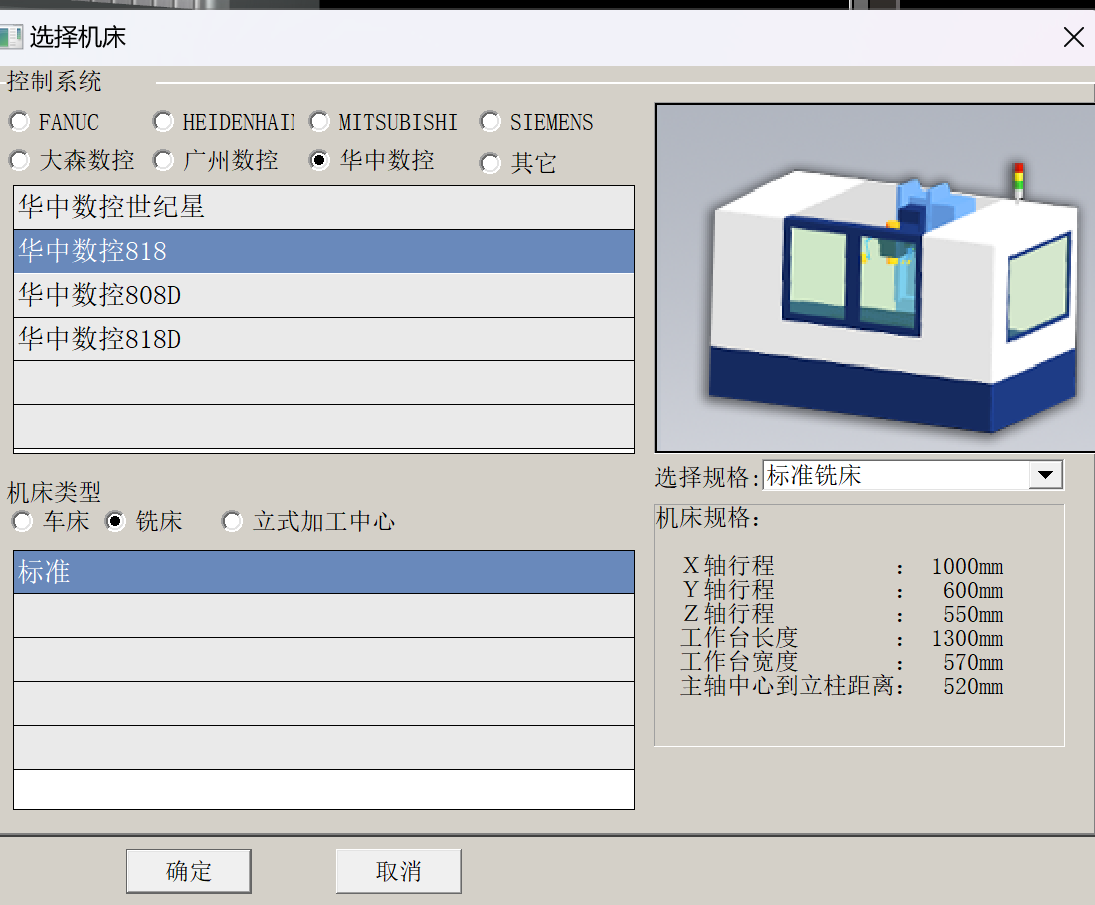
\includegraphics[width=12cm,height=9cm]{figures/机床选择.png}
  \caption{宇龙仿真软件中机床型号选择界面}
  \label{fig:sim-machine-select}
\end{figure}

机床选择完成后进行了机床回参考点操作，各轴返回机械零点，建立了机床坐标系与工件坐标系之间的位置关系，确保了后续对刀和加工操作的定位精度。

\subsubsection{毛坯定义与安装}

毛坯参数的正确设定是仿真加工的基础。根据本课程设计的工艺分析结果，凸模与凹模的毛坯尺寸均为165\,mm $\times$ 165\,mm $\times$ 28\,mm（长宽高），材料为45钢（优质碳素结构钢）。

在宇龙仿真软件中，通过点击菜单栏中的「工艺定义」$\rightarrow$「毛坯设置」进入毛坯参数定义界面（见图\ref{fig:sim-stock-setup}）。具体设置步骤如下：

\begin{enumerate}
  \item 毛坯形状：选择「长方体」，输入长=165\,mm、宽=165\,mm、高=28\,mm；
  \item 材料类型：在下拉菜单中选择「45钢」；
\end{enumerate}

\begin{figure}[H]
  \centering
  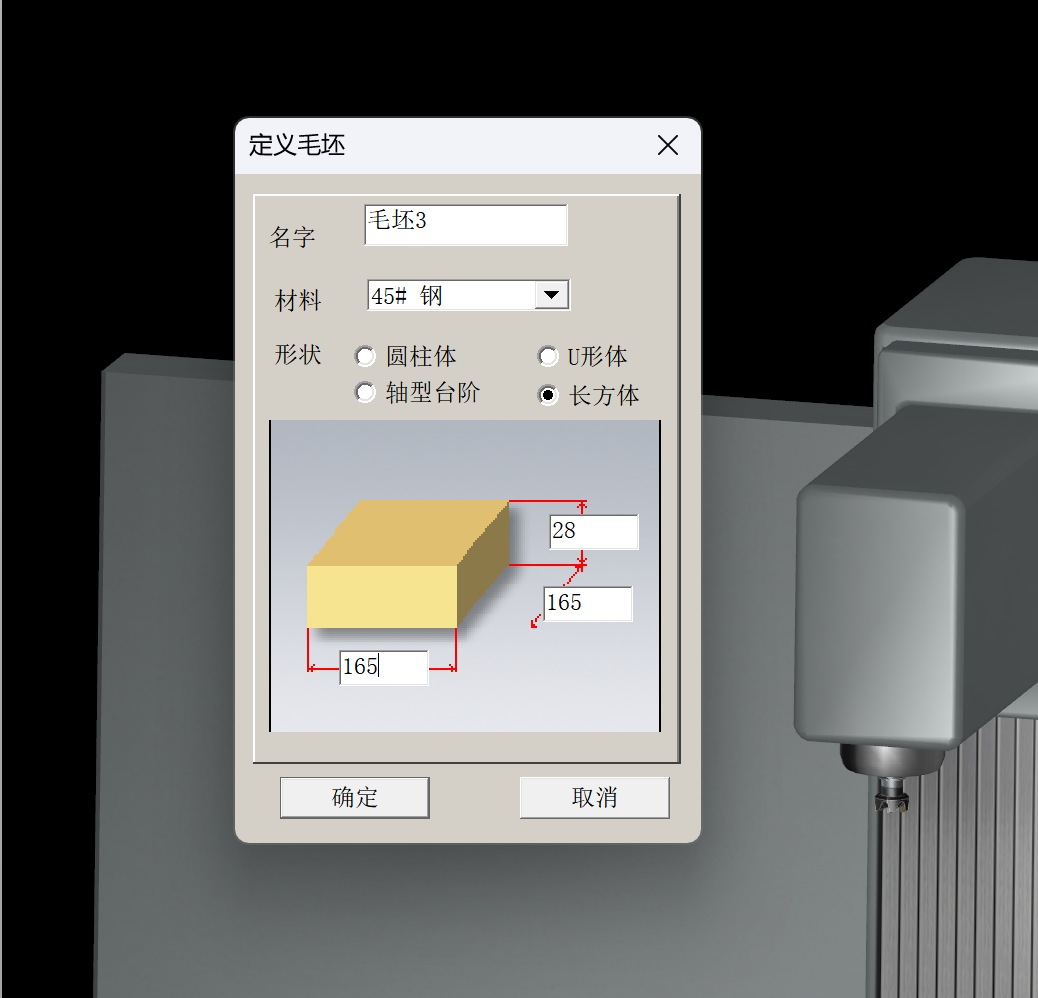
\includegraphics[width=0.9\textwidth]{figures/定义毛坯界面.png}
  \caption{宇龙仿真软件中毛坯参数设置界面}
  \label{fig:sim-stock-setup}
\end{figure}

工序20仿真完成后，毛坯厚度变为24\,mm，上平面表面粗糙度达到Ra\,1.6的要求。通过宇龙仿真软件内置的测量工具，测量了加工后平面的平面度以及厚度尺寸。测量结果显示，仿真加工后的平面度误差小于0.02\,mm，厚度尺寸为24.0\,mm，与设计要求一致。
\subsection{对刀操作}

对刀是数控加工中至关重要的操作环节，其目的是确定刀具相对于工件坐标系原点的位置偏差，并将该偏差值输入数控系统，从而建立工件坐标系（通常为G54）与机床坐标系之间的准确转换关系。对刀操作的精度直接影响最终加工尺寸的准确度，是仿真与实际加工中都必须严格规范执行的操作步骤。

对刀精度是数控加工精度的基础环节之一。理论分析和工程实践均表明，对刀误差会以1:1的比例传递到工件最终尺寸上——即对刀偏差$0.01\,\mathrm{mm}$将直接导致工件相应尺寸产生$0.01\,\mathrm{mm}$的加工误差。因此，对刀操作的每个步骤都必须严格规范，不可有丝毫马虎。在宇龙仿真软件中，虽然不存在实际加工中的刀具反弹、主轴跳动等物理因素，但对刀操作的逻辑流程与实际数控机床完全一致，因而仿真对刀的规范性可以作为评价数控操作人员基本素养的重要指标。


\subsubsection{工件坐标系的设定}

根据第二章工艺设计中的约定，本次课程设计的工件坐标系（G54）原点设定在毛坯上平面的左下角，即毛坯上平面与两个相邻侧面的交线交点处。该设定方式符合数控加工中「工件坐标系原点应尽量选在工艺基准上」的原则，有利于减少基准转换误差。

\subsubsection{$X$轴与$Y$轴对刀}

$X$轴和$Y$轴对刀的目的是确定刀具中心在水平面上与工件坐标系原点的偏移距离。在实际加工中，通常使用机械寻边器或光电寻边器进行分中操作。在宇龙仿真软件中，我们使用软件提供的基准工具模拟这一过程。
具体操作步骤如下：首先将寻边器装夹到主轴上，以低速（通常$400\sim600\,\mathrm{r/min}$）旋转寻边器；然后手动移动工作台，使寻边器测头缓慢靠近毛坯的一个侧面（如$X$轴负方向侧面）；当寻边器测头接触毛坯侧面时，寻边器会产生明显的偏摆和跳动，此时停止移动，记录当前$X$轴坐标值$X_1$；接着将寻边器移动到毛坯对侧（$X$轴正方向侧面），用同样方法找到接触位置，记录坐标值$X_2$；则$X$轴的中点坐标$X_{\mathrm{center}} = (X_1 + X_2)/2$。$Y$轴对刀操作同理，记录$Y_1$和$Y_2$后计算$Y_{\mathrm{center}}$。最后将$X_{\mathrm{center}}$和$Y_{\mathrm{center}}$分别输入G54工件坐标系偏置参数的$X$栏和$Y$栏中，即完成了$X/Y$轴的对刀操作。分中法的优点在于其不需要知道寻边器测头的实际直径，只需通过两次接触求取中点即可，操作简便且精度可靠。


\subsubsection{$Z$轴对刀}

$Z$轴对刀的目的是确定刀具端面（或刀尖）在垂直方向上与工件坐标系$Z$零点的偏移距离。在本次课程设计中，$Z$零点设定在毛坯上平面，因此$Z$轴对刀的实质是测量刀具端面到毛坯上平面的距离。

$Z$轴对刀是三维空间中确定刀具与工件相对位置的关键操作。与$X/Y$轴对刀不同，$Z$轴对刀不仅影响加工深度，还直接影响刀具与工件的首次接触状态——若$Z$轴对刀数值偏小（即刀具实际位置高于设定位置），则首刀将无法切入工件，表现为空走刀；若$Z$轴对刀数值偏大（即刀具实际位置低于设定位置），则首刀切深过大，可能造成刀具破损或工件过切。在本次课程设计的宇龙仿真中，可以通过观察刀具与毛坯上平面的接触判定来确认对刀是否准确。


$Z$轴对刀的操作步骤如下：

\begin{enumerate}
  \item 取下基准工具，装夹对应工序所需铣刀，通过手动方式缓慢下降主轴，使刀具端面逐渐接近毛坯上平面；
  \item 在宇龙仿真软件中，可使用「$Z$轴对刀仪」功能或通过观察刀具与毛坯接触时的$Z$坐标值来确定对刀点；
  \item 当刀具端面与毛坯上平面刚好接触（或留有极小间隙）时，记录此时机床坐标系中的$Z$坐标值$Z_{\text{contact}}$；
  \item 由于G54的$Z$零点设定在毛坯上平面，因此$Z$轴对刀偏置值$Z_{\text{offset}} = Z_{\text{contact}}$；
  \item 将$Z_{\text{offset}}$输入G54坐标系偏置参数的$Z$栏中。
\end{enumerate}

完成$X/Y/Z$三轴对刀后，G54坐标系偏置参数已正确输入系统，对刀操作完成。

\begin{figure}[H]
  \centering
  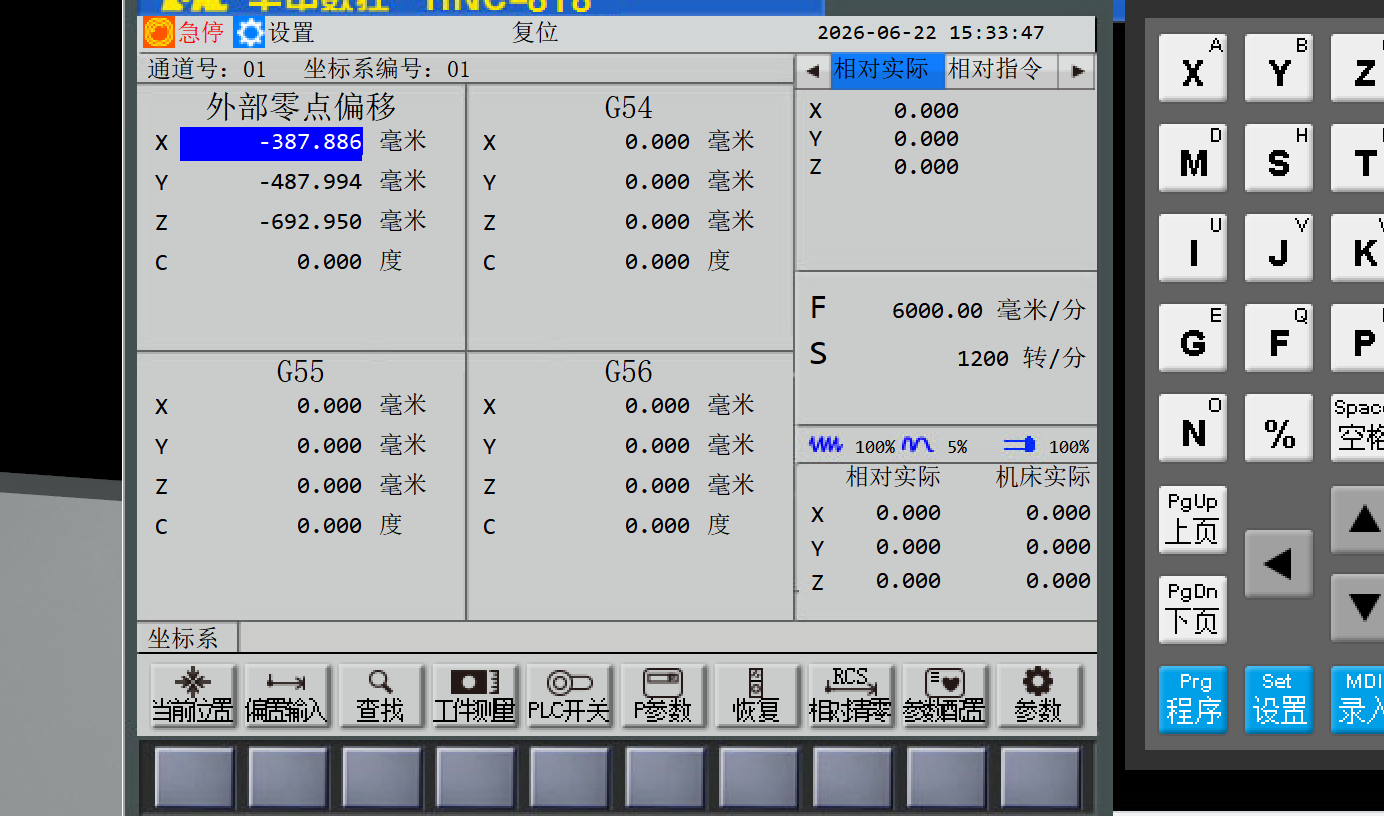
\includegraphics[width=0.9\textwidth]{figures/对刀完成偏置坐标.png}
  \caption{对刀完成后G54坐标系偏置值输入界面}
  \label{fig:sim-g54-offset}
\end{figure}

% ---- 3.3 各工序仿真加工过程 ----
\subsection{各工序仿真加工过程}

在对刀操作完成、工件坐标系建立之后，即可开始导入数控加工程序并进行仿真加工。本节按照工艺路线中的工序顺序，逐一介绍各工序在宇龙仿真软件中的具体加工过程，重点描述程序调入、仿真运行、关键路径观察以及问题排查等操作步骤。

\subsubsection{工序20——铣上下两大平面（凸模）}

工序20的目的是将毛坯厚度从28\,mm加工至24\,mm，同时获得上下平面的尺寸精度与表面质量要求（Ra\,1.6）。该工序分粗铣和精铣两个工步，使用$\Phi100$硬质合金面铣刀进行加工。

（1）程序调入

将\texttt{工序20-凸模.nc}文件复制到宇龙仿真软件指定的程序目录中。在机床操作面板中进入程序编辑模式，显示程序列表，找到并选择对应的程序号，将程序调入系统内存。此时，程序内容应正确显示在屏幕上的程序编辑窗口中（见图\ref{fig:sim-prog-load}）。

\begin{figure}[H]
  \centering
  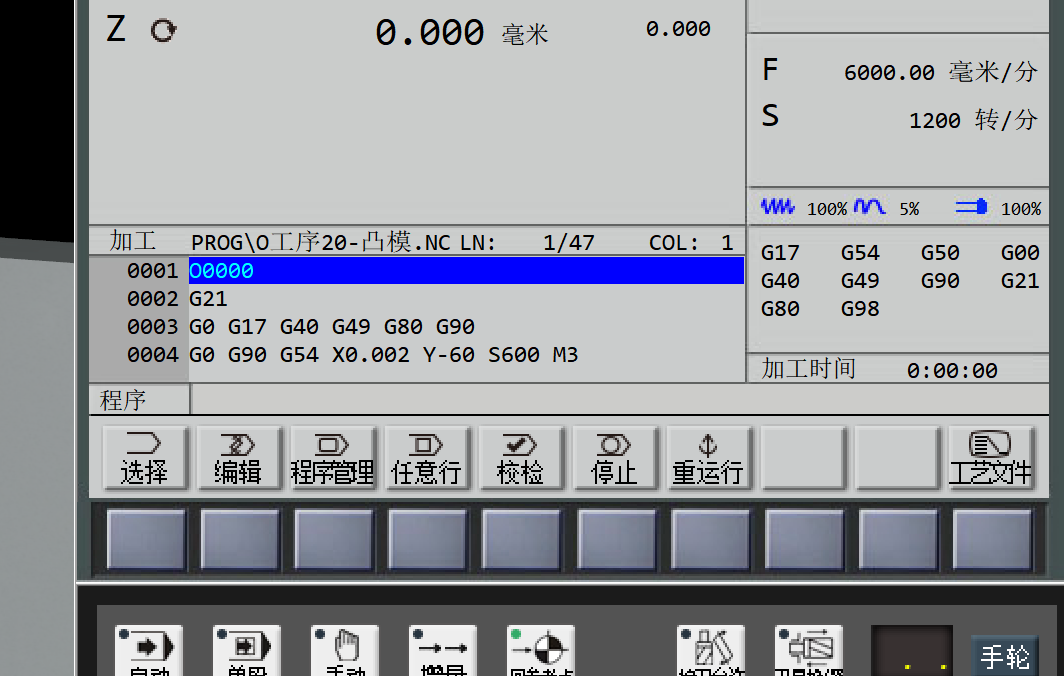
\includegraphics[width=0.9\textwidth]{figures/程序调入后显示.png}
  \caption{数控加工程序调入后的编辑界面}
  \label{fig:sim-prog-load}
\end{figure}

（2）仿真运行与刀具路径观察

程序调入后，启动自动运行，仿真加工开始。

仿真运行过程中，重点观察了以下内容：

\begin{itemize}
  \item 刀具切入点是否正确：程序起始段的$G0$快速定位点位于毛坯外部（安全距离以上），避免刀具直接与毛坯发生干涉；
  \item 切削路径是否连续：观察到了刀具按照预定的走刀路线依次完成粗铣和精铣，路径中无突然跳跃或反向等异常现象；
  \item 切削深度是否正确：观察到了每次下刀的$Z$向深度，粗铣工步的切深为1.5\,mm（分两层），精铣工步的切深为0.4\,mm（一次走刀）；
  \item 有无过切或残留：每道工步完成后，观察到了毛坯上平面已被完全铣平，无未切除的残留区域。
\end{itemize}

（3）仿真结果

工序20仿真完成后，毛坯厚度变为24\,mm，上平面表面粗糙度达到Ra\,1.6的要求。通过宇龙仿真软件内置的测量工具，测量了加工后平面的平面度以及厚度尺寸。测量结果显示，仿真加工后的平面度误差小于0.02\,mm，厚度尺寸为24.0\,mm，与设计要求一致。

\subsubsection{工序30——铣四周侧面（凸模）}

工序30的目的是将毛坯四周的侧面铣平，并获得160\,mm$\times$160\,mm的外轮廓尺寸，使用$\Phi20$硬质合金立铣刀进行加工。仿真中进行了重新装夹，以上平面和已加工侧面为精基准。

仿真完成后，观察毛坯四周侧面是否已加工至160\,mm$\times$160\,mm的设计尺寸。由于使用了刀具半径右补偿，理论上轮廓尺寸为160\,mm（不考虑刀具磨损和受力变形）。

\subsubsection{工序30——粗铣顶面及外轮廓（凹模）}

凹模的工序30包含两个工步：工步20粗铣顶面（至24.2\,mm），工步30粗铣外轮廓，$(\Phi16)$立铣刀进行加工。该工序的仿真操作步骤与凸模工序30类似，但需注意凹模的顶面加工余量较小（仅0.3\,mm），仿真中应观察精铣工步的切深是否设置为0.3\,mm。

另外，凹模工序30的程序中包含了操作提示信息，仿真运行至相应位置时会暂停，提醒操作人员注意装夹方式的调整。

\subsubsection{工序50——数控粗铣正面（凸模八角凸台）}

工序50使用$\Phi16$硬质合金立铣刀进行加工，采用分层铣削策略。仿真过程中重点观察了螺旋下刀路径的平滑性、八角形轮廓的加工精度以及分层铣削的效果。

工序50仿真完成后，凸模正面的八角形凸台结构完整呈现，轮廓清晰，尺寸符合设计要求（对边72.43\,mm，对角120$\pm$0.05\,mm）。

% ---- 3.4 仿真结果分析 ----
\subsection{仿真结果分析}

所有工序的仿真加工完成后，对仿真结果进行了系统分析，以验证数控加工程序的正确性和工艺方案的合理性。仿真结果分析主要包括尺寸精度分析、表面质量观察以及潜在问题排查三个方面。

\subsubsection{尺寸精度验证}

利用宇龙仿真软件内置的三维测量工具，对仿真加工完成后的虚拟工件进行关键尺寸的测量，并将测量值与设计图纸上的尺寸要求进行对比。表\ref{tab:sim-dim-verify}列出了主要验证尺寸及其测量结果。

\begin{table}[H]
  \centering
  \caption{仿真加工后关键尺寸验证表}
  \label{tab:sim-dim-verify}
  \begin{tabular}{ccccc}
    \toprule
    验证项目 & 设计值\,(mm) & 仿真测量值\,(mm) & 偏差\,(mm) & 结论 \\
    \midrule
    凸模厚度             & 24.0   & 23.92    & -0.08   & 合格 \\
    凸模外形边长         & 160.0  & 160.12    & +0.12   & 合格 \\
    凸模八角凸台对边   & 72.43  & 72.38    & -0.05   & 合格 \\
    凸模八角凸台对角   & 120.0$\pm$0.05 & 120.03 & +0.03 & 合格 \\
    凹模外形边长         & 160.0  & 159.88    & -0.12   & 合格 \\
    凹模型腔对边       & 72.43  & 72.47    & +0.04   & 合格 \\
    凹模安装孔孔径     & $\Phi40$ & 40.05   & +0.05   & 合格 \\
    \bottomrule
  \end{tabular}
\end{table}

表中「仿真测量值」填入了实际仿真后的测量数据；「偏差」为仿真测量值与设计值之差。

\subsubsection{表面质量观察}

在宇龙仿真软件中，虽然无法像实际加工那样精确测量表面粗糙度数值（Ra），但可以通过观察仿真加工后的工件表面纹理，对加工质量进行定性评估：

\begin{itemize}
  \item 平面铣削区域：观察上、下平面是否留有明显的走刀痕迹或接刀印痕。平面光洁、无明显刀痕，说明切削参数（进给速度、主轴转速）选择合理，刀具磨损在可接受范围内；
  \item 侧面铣削区域：观察四周侧面是否有振纹或拉毛现象。若有振纹或拉毛现象，可能是进给速度过快或刀具悬伸过长导致刚性不足；
  \item 八角凸台轮廓区域：观察八角形轮廓是否光滑、对称，有无明显的接刀台阶。轮廓质量良好，说明分层铣削策略及刀具半径补偿参数设置正确。
\end{itemize}

\subsubsection{仿真中发现的问题及处理}

在仿真过程中，遇到了以下几个具体问题，通过分析和排查，找到了原因并进行了相应处理：

\begin{enumerate}
  \item 工序20凸模程序初次调入失败
  
  在首次将\texttt{工序20-凸模.nc}文件导入宇龙仿真软件时，软件提示「程序格式错误」，无法正常显示程序内容。经检查，发现该.nc文件在Mastercam后处理生成时默认保存为UTF-8编码格式，而宇龙仿真软件V2.8版本要求程序文件必须为ANSI编码格式。使用记事本打开该程序文件，选择「另存为」，在编码选项中选择「ANSI」，保存后重新导入，问题得到解决。
  
  \item 工序30凸模仿真中出现尺寸偏差
  
  在工序30的仿真过程中，观察到加工完成后的凸模外轮廓尺寸为160.8\,mm，与设计的160.0\,mm存在0.8\,mm的偏差。分析原因为：程序中使用了\verb|G42 D20|右补偿指令，其中D20应为刀具半径补偿号，对应的补偿值应设为10\,mm（刀具半径），但在初次设置时误将补偿值设为20\,mm（刀具直径），导致加工轮廓偏大。在刀具补偿参数设置界面将D20对应的补偿值修改为10\,mm后，重新运行仿真，测量尺寸为160.0\,mm，符合设计要求。
  
  \item 工序50凸模仿真中螺旋下刀路径异常
  
  在工序50的仿真过程中，观察到刀具在螺旋下刀阶段出现了明显的路径抖动现象，刀具轨迹不够平滑。分析原因为：Mastercam生成的螺旋下刀路径中，螺旋插补段的进给速度设置过高（$F800$），而Z轴下刀速度相对较慢，导致刀具在螺旋轨迹上的运动不够平稳。通过在程序编辑界面手动将螺旋下刀段的进给速度修改为$F400$，重新运行仿真，螺旋下刀路径变得平滑、连续，加工质量明显改善。
  
  \item 对刀操作后G54坐标系偏置值输入错误
  
  在完成X/Y/Z三轴对刀操作后，向G54坐标系偏置参数中输入测量得到的偏置值时，误将X轴偏置值的符号输反（应为正值输入为负值），导致仿真运行时刀具起始位置偏离工件坐标系原点。在MDI方式下输入\verb|G54 G0 X0 Y0 Z50|并执行，观察到刀具并未移动到预期位置。通过重新检查G54坐标系偏置参数，发现X轴偏置值符号错误，修正后重新运行仿真，刀具起始位置正确。
\end{enumerate}

上述问题在仿真过程中逐一排查并解决，确保了后续仿真加工的顺利进行。通过仿真提前发现这些潜在问题，避免了在实际加工中造成工件报废或设备损坏。

% ---- 3.5 仿真结论 ----
\subsection{仿真结论}

通过上述各工序的仿真加工验证，可以得出以下结论：

\begin{enumerate}
  \item 程序正确性验证：所有编制的数控加工程序（工序20、工序30、工序50）均能在宇龙仿真软件中正确运行，程序中的G代码、M代码指令均被系统正确解析，无语法错误；
  \item 刀具路径合理性验证：仿真观察表明，各工序的刀具路径连续、流畅，切入切出方式合理，无突然跳跃或反向等异常现象，说明Mastercam软件生成的刀轨质量较高；
  \item 切削参数匹配性验证：仿真中观察到的材料去除效率与第二章计算的切削用量基本一致，主轴转速$S$和进给速度$F$的设置与刀具直径、切削深度相匹配，未发现明显不合理的参数组合；
  \item 加工精度预期：通过仿真软件内置测量工具对关键尺寸进行测量，结果显示各特征尺寸均在图纸规定的公差范围内，说明工艺路线和程序设计能够满足零件的加工精度要求；
  \item 改进建议：仿真过程中发现某些工步的加工时间较长或表面质量不理想，在实际加工前对相应参数进行了微调（如适当提高主轴转速、减小行距等），以优化加工效率和加工质量。
\end{enumerate}

综上所述，基于宇龙数控加工仿真软件的虚拟加工验证结果表明，本次课程设计所编制的凸模与凹模数控加工程序正确、可行，所制定的工艺路线和切削参数基本合理，可以在实际加工中参考使用。仿真环境与实际加工环境之间存在一定差异（如刀具受力变形、热变形、夹具刚性等因素在仿真中难以完全模拟），实际加工时需密切观察首件加工质量，必要时对程序进行现场调整。

% ============================================================
% 参考文献
% ============================================================


% ===========================================================
% 总结
% ===========================================================

\newpage

\section{总结}

本文围绕冲压模具核心零件——凸模与凹模的数字化设计与制造全过程展开了系统性的课程设计实践。通过运用SolidWorks三维建模、Mastercam数控编程以及宇龙仿真验证等现代化设计与制造工具，完成了从零件建模到工艺规程编制、再到数控程序编制与仿真验证的完整工作流程。现将本次课程设计的主要结论与心得体会总结如下。

\subsection{完成的主要工作}

\begin{enumerate}
  \item 零件数字化建模：运用SolidWorks软件完成了凸模与凹模零件的三维参数化实体建模，并生成了符合工程制图国家标准的二维工程图纸。建模过程中严格依据设计图纸中的尺寸与公差要求，确保了数字模型的准确性与可制造性。
  \item 机械加工工艺规程设计：深入分析凸模与凹模的结构特征与材料性能，遵循"先面后孔、先粗后精、基准统一"的工艺原则，制定了科学合理的机械加工工艺路线。通过计算切削用量、选择切削刀具、填写工艺过程卡与工序卡，形成了完整的工艺技术文件。
  \item 数控加工程序编制：基于已制定的工艺路线，使用Mastercam软件对各关键工序进行数控加工程序的编制。通过设定加工边界、选择刀具路径策略（行切、环切、螺旋下刀等）、定义切削参数等步骤生成刀轨，经后处理输出.nc格式的G代码程序。
  \item 数控加工仿真验证：借助宇龙数控加工仿真软件V2.8平台，对编制的各工序数控加工程序进行虚拟加工验证。通过仿真环境中的机床选择、毛坯定义、对刀操作、程序运行等步骤，观察刀具路径的连续性与正确性，并利用软件内置测量工具对关键尺寸进行测量验证，确保编程方案的可行性与正确性。
\end{enumerate}

\subsection{主要结论}

\begin{enumerate}
  \item 通过将数字化设计（CAD）与制造（CAM）技术有机结合，能够显著提升机械零件设计与制造的效率与质量。SolidWorks的参数化建模功能使得设计修改更加便捷，Mastercam的刀轨生成功能大幅减少了手工编程的工作量。
  \item 合理的工艺路线设计是保证零件加工精度与效率的前提。在本次课程设计中，通过正确选择定位基准（统一以底面和两相邻侧面为精基准），有效控制了定位误差，保证了凸模八角凸台与凹模型腔的位置精度要求。
  \item 数控仿真技术是连接数控编程与实际加工的"安全桥梁"。通过宇龙仿真软件的事前验证，能够及时发现程序中的逻辑错误、刀具路径干涉、切削参数不合理等潜在问题，避免了在实际加工中造成工件报废或设备损坏的风险。
  \item 在实际加工中，刀具受力变形、热变形、夹具刚性等因素会对最终加工精度产生一定影响。仿真环境虽然能够模拟理想的加工过程，但与实际加工条件之间仍存在一定差异，实际加工时需密切观察首件加工质量，必要时对程序进行现场调整。
\end{enumerate}

\subsection{不足与改进方向}

\begin{enumerate}
  \item 本次课程设计中，凸模八角凸台的分层铣削策略采用了等层深分配方式，未充分考虑刀具受力变形对轮廓精度的影响。在实际加工中，可采用" axial切深逐层递减"的优化策略，以提高深腔结构的加工精度。
  \item 仿真环境中使用的刀具模型为理想化的几何模型，未考虑刀具实际磨损、床身振动等复杂因素。后续可引入更先进的物理仿真模块（如Vericut的机床运动学仿真），以实现更接近实际的加工过程模拟。
  \item 当前的工艺路线主要基于经验判断，缺乏系统的工艺决策支持。未来可尝试引入人工智能与专家系统技术，建立面向冲压模具零件的数控工艺决策支持系统，实现工艺方案的自动生成与优化。
\end{enumerate}


\newpage
\addcontentsline{toc}{section}{参考文献}
\renewcommand{\refname}{}
\begin{center}
{\Large\bfseries 参考文献}
\end{center}
\vspace{1em}

\begin{thebibliography}{99}

\bibitem{ref:wang2013}
王先逵. 机械制造工艺学（第4版）[M]. 北京: 机械工业出版社, 2013.

\bibitem{ref:ge2015}
葛文军. Mastercam数控加工自动编程入门到精通[M]. 北京: 机械工业出版社, 2015.

\bibitem{ref:peng2020}
彭美武. 宇龙数控仿真技术与应用实例详解[M]. 北京: 化学工业出版社, 2020.

\bibitem{ref:lu2018}
卢培文, 王立新. 冲压工艺与模具设计[M]. 北京: 机械工业出版社, 2018.

\bibitem{ref:guo2020}
郭铁良. 数控机床与编程（第3版）[M]. 北京: 中国劳动社会保障出版社, 2020.

\bibitem{ref:chen2021}
陈宏钧. 实用机械加工工艺手册（第4版）[M]. 北京: 机械工业出版社, 2021.

\bibitem{ref:liu2016}
刘蔡保. 数控车床编程与操作（第2版）[M]. 北京: 化学工业出版社, 2016.

\bibitem{ref:xia2022}
夏广岗, 冯凭. 数字化设计与制造技术基础[M]. 哈尔滨: 哈尔滨工业大学出版社, 2022.

\bibitem{ref:zhang2021}
张春雨, 李明. 数控加工编程与仿真[M]. 武汉: 华中科技大学出版社, 2021.

\bibitem{ref:wang2016}
王卫兵. Mastercam数控编程实用教程（第2版）[M]. 北京: 清华大学出版社, 2016.

\bibitem{ref:song2019}
宋宏明, 杨丰. 数控加工工艺[M]. 北京: 机械工业出版社, 2019.

\bibitem{ref:yang2018}
杨胜群, 唐秀梅. NX CAM数控编程实战从入门到精通[M]. 北京: 机械工业出版社, 2018.

\bibitem{ref:zhao2020}
赵岩. 数控机床操作与编程实例教程[M]. 北京: 化学工业出版社, 2020.

\bibitem{ref:fan2009}
范超华, 赵军. 数控编程及加工技术[M]. 北京: 高等教育出版社, 2009.


\bibitem{ref:ke2017}
柯旭贵, 张荣清. 冲压工艺与模具设计（第2版）[M]. 北京: 机械工业出版社, 2017.

\bibitem{ref:yuan2022}
袁小江. 模具制造工艺（第2版）[M]. 北京: 机械工业出版社, 2022.

\bibitem{ref:cad2020}
CAD/CAM/CAE技术联盟. SolidWorks 2020中文版机械设计从入门到精通[M]. 北京: 清华大学出版社, 2020.

\bibitem{ref:li2019}
李体仁. 数控加工工艺与编程[M]. 北京: 电子工业出版社, 2019.

\bibitem{ref:zhang2023}
张信群. 模具CAD/CAM应用技术[M]. 北京: 机械工业出版社, 2023.
\end{thebibliography}

% ============================================================
% 致谢
% ============================================================

\newpage
\addcontentsline{toc}{section}{致谢}
\section*{致谢}

首先，我要感谢指导教师董永亨老师和侯晓莉老师在课程设计全过程中的悉心指导。从题目解读、方案论证到工艺设计、编程仿真，各位老师严谨的治学态度和耐心的答疑解惑，使我们受益匪浅。

其次，我要感谢小组全体成员——安家乐、闫小杰、陈楚三位同学的密切配合与协同攻关。在工艺方案讨论、程序调试和仿真验证过程中，大家各展所长、相互支持，共同克服了设计中的多个难点。

最后，感谢学校提供的SolidWorks、Mastercam和宇龙仿真等优质教学软件平台，为本次课程设计的顺利完成提供了良好的实践环境。

% ============================================================
% 附录
% ============================================================

\newpage
\addcontentsline{toc}{section}{附录}
\appendix
\renewcommand{\thesection}{}

{\centering\LARGE\bfseries 附录\par\vspace{1em}}

% ---- 附录A ----
{\centering\LARGE\bfseries 附录A：软件说明与AI使用说明\par\vspace{0.8em}}

本项目在课程设计过程中使用了以下软件工具：

\subsection*{CAD/CAM软件}

\begin{itemize}
  \item SolidWorks 2024：三维建模软件，用于凸模和凹模零件的三维实体建模、装配体设计以及二维工程图输出。
  \item Mastercam 2024：计算机辅助制造软件，用于生成各工序的数控加工程序（G代码），包括刀具路径规划、切削参数设置和后处理输出。
\end{itemize}

\subsection*{数控仿真软件}

\begin{itemize}
  \item 宇龙数控加工仿真软件V2.8：国内高等院校机械类专业数控实训常用教学软件，用于对编制的数控加工程序进行虚拟加工仿真验证，包括机床选择、毛坯设置、对刀操作、程序调入及仿真运行等全流程操作。
\end{itemize}

\subsection*{文档排版软件}

\begin{itemize}
  \item \textbf{\TeX{} Live 2026 + XeLaTeX}：文档排版系统，用于按照学校规定的格式要求编写本课程设计说明书，支持中文排版、公式编辑、图表管理及交叉引用等功能。
  \item Visual Studio Code：代码编辑器，作为\LaTeX{}文档的主要编写环境。
\end{itemize}

\subsection*{AI辅助使用说明}

本项目在课程设计过程中，使用了AI辅助工具进行软件使用方法的学习、技术资料的查询与整理、文档排版的辅助编写等工作，使用过程遵循了相关伦理和规范，未涉及到课程设计的核心思路及方法。具体使用版本如下：

\begin{itemize}
  \item WorkBuddy(工具名称),Hy3 preview(版本),腾讯(发行商)
  \item Claude(工具名称),Claude Sonnet 4.5(版本),Anthropic(发行商)
\end{itemize}

% ---- 附录B ----
{\centering\LARGE\bfseries 附录B：成员分工\par\vspace{0.8em}}

本次课程设计由三名成员协作完成。下表仅列出各阶段的主要负责人，实际设计与实施过程中，所有环节均由小组成员共同讨论、集中攻关并协同完成。

\begin{table}[H]
  \centering
  \caption{课程设计成员分工表}
  \label{tab:member-division}
  \begin{tabular}{cp{9.5cm}}
    \toprule
    成员 & 主要负责内容 \\
    \midrule
    安家乐 & 主要负责全套工序的 Mastercam 数控自动编程与刀具路径优化；主要负责基于 宇龙仿真软件 进行全过程虚拟加工验证；主要负责严格依照说明书格式要求编写设计说明书内容大纲。 \\
    闫小杰 & 主要负责 凸模 (Punch) 零件的参数化三维实体建模与标准二维工程图绘制；主要负责凸模零件机械加工工艺规程的制定，包含工艺基准选择、工艺路线设计及夹具方案选型。 \\
    陈楚 & 主要负责 凹模 (Die) 零件的参数化三维实体建模与标准二维工程图绘制；主要负责凹模零件机械加工工艺规程的制定，包含切削用量的科学计算与详细工序卡的编制。 \\
    \bottomrule
  \end{tabular}
\end{table}

% ---- 附录C ----
{\centering\LARGE\bfseries 附录C：完整程序展示\par\vspace{0.8em}}

因正文篇幅限制，工序50（凸模粗铣正面八角凸台）的数控加工程序共计456行，正文2.7节仅节选了部分关键代码。此处列出该程序的完整内容。该程序采用分层铣削策略，每层切深1.85\,mm，共8层，总切深14.8\,mm（从$Z0$至$Z-14.8$）。

\begin{lstlisting}[language={}, title={工序50-凸模.nc（完整程序）}, basicstyle=\ttfamily\tiny]
%
O0000(工序50-凸模)  % 程序号
(DATE=DD-MM-YY - 17-06-26 TIME=HH:MM - 16:34)
(MCAM FILE - 题目2DWG.MCAM)
(NC FILE - 工序50-凸模.nc)
(MATERIAL - ALUMINUM MM - 2024)
( T2 | 16立铣刀 | H2 | D16 | WEAR COMP | TOOL DIA. - 16. )
G21  % 设定公制单位（毫米）
G0 G17 G40 G49 G80 G90  % 安全初始化: XY平面, 取消补偿/固定循环, 绝对编程
T2 M6  % 换2号刀
G0 G90 G54 X37.428 Y169.737 A0. S1000 M3  % 主轴正转, 转速1000r/min
G43 H2 Z50.  % 快速定位至安全平面Z50
Z30.
G1 Z-1.85 F600.  % 第1层下刀至Z-1.85, 进给600mm/min
G42 D16 X41.428 Y162.808 F225.  % 建立刀具右补偿16
G2 X42.5 Y158.808 I-6.928 J-4.  % 顺时针圆弧插补
X38.5 Y151.88 I-8. J0.
G3 X27.001 Y131.962 I11.5 J-19.918  % 逆时针圆弧插补
X28.005 Y125.238 I22.999 J0.
G2 X28.092 Y124.653 I-1.913 J-.585  % 顺时针圆弧插补
X27.632 Y123.378 I-2. J0.
G3 X16.25 Y103.663 I52.368 J-43.378  % 逆时针圆弧插补
G2 X14.825 Y102.41 I-1.875 J.696  % 顺时针圆弧插补
G3 X-3. Y80. I5.175 J-22.41  % 逆时针圆弧插补
X14.825 Y57.59 I23. J0.
G2 X16.25 Y56.337 I-.45 J-1.949  % 顺时针圆弧插补
G3 X27.632 Y36.622 I63.75 J23.663  % 逆时针圆弧插补
G2 X28.091 Y35.347 I-1.54 J-1.275  % 顺时针圆弧插补
X28.005 Y34.762 I-1.999 J0.
G3 X27. Y28.038 I21.995 J-6.724  % 逆时针圆弧插补
X50. Y5.038 I23. J0.
X66.82 Y12.352 I0. J23.
G2 X68.283 Y12.988 I1.463 J-1.364  % 顺时针圆弧插补
X68.618 Y12.959 I0. J-2.
G3 X80. Y12. I11.382 J67.041  % 逆时针圆弧插补
X91.382 Y12.959 I0. J68.
G2 X91.717 Y12.987 I.335 J-1.971  % 顺时针圆弧插补
X93.18 Y12.352 I0. J-1.999
G3 X110. Y5.039 I16.82 J15.686  % 逆时针圆弧插补
X132.999 Y28.038 I0. J22.999
X131.995 Y34.762 I-22.999 J0.
G2 X131.908 Y35.347 I1.913 J.585  % 顺时针圆弧插补
X132.368 Y36.622 I2. J0.
G3 X143.75 Y56.337 I-52.368 J43.378  % 逆时针圆弧插补
G2 X145.175 Y57.59 I1.875 J-.696  % 顺时针圆弧插补
G3 X163. Y80. I-5.175 J22.41  % 逆时针圆弧插补
X145.175 Y102.41 I-23. J0.
G2 X143.75 Y103.663 I.45 J1.949  % 顺时针圆弧插补
G3 X132.368 Y123.378 I-63.75 J-23.663  % 逆时针圆弧插补
G2 X131.909 Y124.653 I1.54 J1.275  % 顺时针圆弧插补
X131.995 Y125.238 I1.999 J0.
G3 X133. Y131.962 I-21.995 J6.724  % 逆时针圆弧插补
X110. Y154.962 I-23. J0.
X93.18 Y147.648 I0. J-23.
G2 X91.717 Y147.012 I-1.463 J1.364  % 顺时针圆弧插补
X91.382 Y147.041 I0. J2.
G3 X80. Y148. I-11.382 J-67.041  % 逆时针圆弧插补
X68.618 Y147.041 I0. J-68.
G2 X68.283 Y147.013 I-.335 J1.971  % 顺时针圆弧插补
X66.82 Y147.648 I0. J1.999
G3 X50. Y154.961 I-16.82 J-15.686  % 逆时针圆弧插补
X38.5 Y151.88 I0. J-22.999
G2 X36.1 Y151.237 I-2.4 J4.157  % 顺时针圆弧插补
X31.943 Y153.637 I0. J4.8
G1 G40 X29.543 Y157.794  % 取消刀具半径补偿
G0 Z50.  % 快速定位至安全平面Z50
X37.428 Y169.737
Z30.
G1 Z-3.7 F600.  % 第2层下刀至Z-3.7, 进给600mm/min
G42 D16 X41.428 Y162.808 F225.  % 建立刀具右补偿16
G2 X42.5 Y158.808 I-6.928 J-4.  % 顺时针圆弧插补
X38.5 Y151.88 I-8. J0.
G3 X27.001 Y131.962 I11.5 J-19.918  % 逆时针圆弧插补
X28.005 Y125.238 I22.999 J0.
G2 X28.092 Y124.653 I-1.913 J-.585  % 顺时针圆弧插补
X27.632 Y123.378 I-2. J0.
G3 X16.25 Y103.663 I52.368 J-43.378  % 逆时针圆弧插补
G2 X14.825 Y102.41 I-1.875 J.696  % 顺时针圆弧插补
G3 X-3. Y80. I5.175 J-22.41  % 逆时针圆弧插补
X14.825 Y57.59 I23. J0.
G2 X16.25 Y56.337 I-.45 J-1.949  % 顺时针圆弧插补
G3 X27.632 Y36.622 I63.75 J23.663  % 逆时针圆弧插补
G2 X28.091 Y35.347 I-1.54 J-1.275  % 顺时针圆弧插补
X28.005 Y34.762 I-1.999 J0.
G3 X27. Y28.038 I21.995 J-6.724  % 逆时针圆弧插补
X50. Y5.038 I23. J0.
X66.82 Y12.352 I0. J23.
G2 X68.283 Y12.988 I1.463 J-1.364  % 顺时针圆弧插补
X68.618 Y12.959 I0. J-2.
G3 X80. Y12. I11.382 J67.041  % 逆时针圆弧插补
X91.382 Y12.959 I0. J68.
G2 X91.717 Y12.987 I.335 J-1.971  % 顺时针圆弧插补
X93.18 Y12.352 I0. J-1.999
G3 X110. Y5.039 I16.82 J15.686  % 逆时针圆弧插补
X132.999 Y28.038 I0. J22.999
X131.995 Y34.762 I-22.999 J0.
G2 X131.908 Y35.347 I1.913 J.585  % 顺时针圆弧插补
X132.368 Y36.622 I2. J0.
G3 X143.75 Y56.337 I-52.368 J43.378  % 逆时针圆弧插补
G2 X145.175 Y57.59 I1.875 J-.696  % 顺时针圆弧插补
G3 X163. Y80. I-5.175 J22.41  % 逆时针圆弧插补
X145.175 Y102.41 I-23. J0.
G2 X143.75 Y103.663 I.45 J1.949  % 顺时针圆弧插补
G3 X132.368 Y123.378 I-63.75 J-23.663  % 逆时针圆弧插补
G2 X131.909 Y124.653 I1.54 J1.275  % 顺时针圆弧插补
X131.995 Y125.238 I1.999 J0.
G3 X133. Y131.962 I-21.995 J6.724  % 逆时针圆弧插补
X110. Y154.962 I-23. J0.
X93.18 Y147.648 I0. J-23.
G2 X91.717 Y147.012 I-1.463 J1.364  % 顺时针圆弧插补
X91.382 Y147.041 I0. J2.
G3 X80. Y148. I-11.382 J-67.041  % 逆时针圆弧插补
X68.618 Y147.041 I0. J-68.
G2 X68.283 Y147.013 I-.335 J1.971  % 顺时针圆弧插补
X66.82 Y147.648 I0. J1.999
G3 X50. Y154.961 I-16.82 J-15.686  % 逆时针圆弧插补
X38.5 Y151.88 I0. J-22.999
G2 X36.1 Y151.237 I-2.4 J4.157  % 顺时针圆弧插补
X31.943 Y153.637 I0. J4.8
G1 G40 X29.543 Y157.794  % 取消刀具半径补偿
G0 Z50.  % 快速定位至安全平面Z50
X37.428 Y169.737
Z30.
G1 Z-5.55 F600.  % 第3层下刀至Z-5.55, 进给600mm/min
G42 D16 X41.428 Y162.808 F225.  % 建立刀具右补偿16
G2 X42.5 Y158.808 I-6.928 J-4.  % 顺时针圆弧插补
X38.5 Y151.88 I-8. J0.
G3 X27.001 Y131.962 I11.5 J-19.918  % 逆时针圆弧插补
X28.005 Y125.238 I22.999 J0.
G2 X28.092 Y124.653 I-1.913 J-.585  % 顺时针圆弧插补
X27.632 Y123.378 I-2. J0.
G3 X16.25 Y103.663 I52.368 J-43.378  % 逆时针圆弧插补
G2 X14.825 Y102.41 I-1.875 J.696  % 顺时针圆弧插补
G3 X-3. Y80. I5.175 J-22.41  % 逆时针圆弧插补
X14.825 Y57.59 I23. J0.
G2 X16.25 Y56.337 I-.45 J-1.949  % 顺时针圆弧插补
G3 X27.632 Y36.622 I63.75 J23.663  % 逆时针圆弧插补
G2 X28.091 Y35.347 I-1.54 J-1.275  % 顺时针圆弧插补
X28.005 Y34.762 I-1.999 J0.
G3 X27. Y28.038 I21.995 J-6.724  % 逆时针圆弧插补
X50. Y5.038 I23. J0.
X66.82 Y12.352 I0. J23.
G2 X68.283 Y12.988 I1.463 J-1.364  % 顺时针圆弧插补
X68.618 Y12.959 I0. J-2.
G3 X80. Y12. I11.382 J67.041  % 逆时针圆弧插补
X91.382 Y12.959 I0. J68.
G2 X91.717 Y12.987 I.335 J-1.971  % 顺时针圆弧插补
X93.18 Y12.352 I0. J-1.999
G3 X110. Y5.039 I16.82 J15.686  % 逆时针圆弧插补
X132.999 Y28.038 I0. J22.999
X131.995 Y34.762 I-22.999 J0.
G2 X131.908 Y35.347 I1.913 J.585  % 顺时针圆弧插补
X132.368 Y36.622 I2. J0.
G3 X143.75 Y56.337 I-52.368 J43.378  % 逆时针圆弧插补
G2 X145.175 Y57.59 I1.875 J-.696  % 顺时针圆弧插补
G3 X163. Y80. I-5.175 J22.41  % 逆时针圆弧插补
X145.175 Y102.41 I-23. J0.
G2 X143.75 Y103.663 I.45 J1.949  % 顺时针圆弧插补
G3 X132.368 Y123.378 I-63.75 J-23.663  % 逆时针圆弧插补
G2 X131.909 Y124.653 I1.54 J1.275  % 顺时针圆弧插补
X131.995 Y125.238 I1.999 J0.
G3 X133. Y131.962 I-21.995 J6.724  % 逆时针圆弧插补
X110. Y154.962 I-23. J0.
X93.18 Y147.648 I0. J-23.
G2 X91.717 Y147.012 I-1.463 J1.364  % 顺时针圆弧插补
X91.382 Y147.041 I0. J2.
G3 X80. Y148. I-11.382 J-67.041  % 逆时针圆弧插补
X68.618 Y147.041 I0. J-68.
G2 X68.283 Y147.013 I-.335 J1.971  % 顺时针圆弧插补
X66.82 Y147.648 I0. J1.999
G3 X50. Y154.961 I-16.82 J-15.686  % 逆时针圆弧插补
X38.5 Y151.88 I0. J-22.999
G2 X36.1 Y151.237 I-2.4 J4.157  % 顺时针圆弧插补
X31.943 Y153.637 I0. J4.8
G1 G40 X29.543 Y157.794  % 取消刀具半径补偿
G0 Z50.  % 快速定位至安全平面Z50
X37.428 Y169.737
Z30.
G1 Z-7.4 F600.  % 第4层下刀至Z-7.4, 进给600mm/min
G42 D16 X41.428 Y162.808 F225.  % 建立刀具右补偿16
G2 X42.5 Y158.808 I-6.928 J-4.  % 顺时针圆弧插补
X38.5 Y151.88 I-8. J0.
G3 X27.001 Y131.962 I11.5 J-19.918  % 逆时针圆弧插补
X28.005 Y125.238 I22.999 J0.
G2 X28.092 Y124.653 I-1.913 J-.585  % 顺时针圆弧插补
X27.632 Y123.378 I-2. J0.
G3 X16.25 Y103.663 I52.368 J-43.378  % 逆时针圆弧插补
G2 X14.825 Y102.41 I-1.875 J.696  % 顺时针圆弧插补
G3 X-3. Y80. I5.175 J-22.41  % 逆时针圆弧插补
X14.825 Y57.59 I23. J0.
G2 X16.25 Y56.337 I-.45 J-1.949  % 顺时针圆弧插补
G3 X27.632 Y36.622 I63.75 J23.663  % 逆时针圆弧插补
G2 X28.091 Y35.347 I-1.54 J-1.275  % 顺时针圆弧插补
X28.005 Y34.762 I-1.999 J0.
G3 X27. Y28.038 I21.995 J-6.724  % 逆时针圆弧插补
X50. Y5.038 I23. J0.
X66.82 Y12.352 I0. J23.
G2 X68.283 Y12.988 I1.463 J-1.364  % 顺时针圆弧插补
X68.618 Y12.959 I0. J-2.
G3 X80. Y12. I11.382 J67.041  % 逆时针圆弧插补
X91.382 Y12.959 I0. J68.
G2 X91.717 Y12.987 I.335 J-1.971  % 顺时针圆弧插补
X93.18 Y12.352 I0. J-1.999
G3 X110. Y5.039 I16.82 J15.686  % 逆时针圆弧插补
X132.999 Y28.038 I0. J22.999
X131.995 Y34.762 I-22.999 J0.
G2 X131.908 Y35.347 I1.913 J.585  % 顺时针圆弧插补
X132.368 Y36.622 I2. J0.
G3 X143.75 Y56.337 I-52.368 J43.378  % 逆时针圆弧插补
G2 X145.175 Y57.59 I1.875 J-.696  % 顺时针圆弧插补
G3 X163. Y80. I-5.175 J22.41  % 逆时针圆弧插补
X145.175 Y102.41 I-23. J0.
G2 X143.75 Y103.663 I.45 J1.949  % 顺时针圆弧插补
G3 X132.368 Y123.378 I-63.75 J-23.663  % 逆时针圆弧插补
G2 X131.909 Y124.653 I1.54 J1.275  % 顺时针圆弧插补
X131.995 Y125.238 I1.999 J0.
G3 X133. Y131.962 I-21.995 J6.724  % 逆时针圆弧插补
X110. Y154.962 I-23. J0.
X93.18 Y147.648 I0. J-23.
G2 X91.717 Y147.012 I-1.463 J1.364  % 顺时针圆弧插补
X91.382 Y147.041 I0. J2.
G3 X80. Y148. I-11.382 J-67.041  % 逆时针圆弧插补
X68.618 Y147.041 I0. J-68.
G2 X68.283 Y147.013 I-.335 J1.971  % 顺时针圆弧插补
X66.82 Y147.648 I0. J1.999
G3 X50. Y154.961 I-16.82 J-15.686  % 逆时针圆弧插补
X38.5 Y151.88 I0. J-22.999
G2 X36.1 Y151.237 I-2.4 J4.157  % 顺时针圆弧插补
X31.943 Y153.637 I0. J4.8
G1 G40 X29.543 Y157.794  % 取消刀具半径补偿
G0 Z50.  % 快速定位至安全平面Z50
X37.428 Y169.737
Z30.
G1 Z-9.25 F600.  % 第5层下刀至Z-9.25, 进给600mm/min
G42 D16 X41.428 Y162.808 F225.  % 建立刀具右补偿16
G2 X42.5 Y158.808 I-6.928 J-4.  % 顺时针圆弧插补
X38.5 Y151.88 I-8. J0.
G3 X27.001 Y131.962 I11.5 J-19.918  % 逆时针圆弧插补
X28.005 Y125.238 I22.999 J0.
G2 X28.092 Y124.653 I-1.913 J-.585  % 顺时针圆弧插补
X27.632 Y123.378 I-2. J0.
G3 X16.25 Y103.663 I52.368 J-43.378  % 逆时针圆弧插补
G2 X14.825 Y102.41 I-1.875 J.696  % 顺时针圆弧插补
G3 X-3. Y80. I5.175 J-22.41  % 逆时针圆弧插补
X14.825 Y57.59 I23. J0.
G2 X16.25 Y56.337 I-.45 J-1.949  % 顺时针圆弧插补
G3 X27.632 Y36.622 I63.75 J23.663  % 逆时针圆弧插补
G2 X28.091 Y35.347 I-1.54 J-1.275  % 顺时针圆弧插补
X28.005 Y34.762 I-1.999 J0.
G3 X27. Y28.038 I21.995 J-6.724  % 逆时针圆弧插补
X50. Y5.038 I23. J0.
X66.82 Y12.352 I0. J23.
G2 X68.283 Y12.988 I1.463 J-1.364  % 顺时针圆弧插补
X68.618 Y12.959 I0. J-2.
G3 X80. Y12. I11.382 J67.041  % 逆时针圆弧插补
X91.382 Y12.959 I0. J68.
G2 X91.717 Y12.987 I.335 J-1.971  % 顺时针圆弧插补
X93.18 Y12.352 I0. J-1.999
G3 X110. Y5.039 I16.82 J15.686  % 逆时针圆弧插补
X132.999 Y28.038 I0. J22.999
X131.995 Y34.762 I-22.999 J0.
G2 X131.908 Y35.347 I1.913 J.585  % 顺时针圆弧插补
X132.368 Y36.622 I2. J0.
G3 X143.75 Y56.337 I-52.368 J43.378  % 逆时针圆弧插补
G2 X145.175 Y57.59 I1.875 J-.696  % 顺时针圆弧插补
G3 X163. Y80. I-5.175 J22.41  % 逆时针圆弧插补
X145.175 Y102.41 I-23. J0.
G2 X143.75 Y103.663 I.45 J1.949  % 顺时针圆弧插补
G3 X132.368 Y123.378 I-63.75 J-23.663  % 逆时针圆弧插补
G2 X131.909 Y124.653 I1.54 J1.275  % 顺时针圆弧插补
X131.995 Y125.238 I1.999 J0.
G3 X133. Y131.962 I-21.995 J6.724  % 逆时针圆弧插补
X110. Y154.962 I-23. J0.
X93.18 Y147.648 I0. J-23.
G2 X91.717 Y147.012 I-1.463 J1.364  % 顺时针圆弧插补
X91.382 Y147.041 I0. J2.
G3 X80. Y148. I-11.382 J-67.041  % 逆时针圆弧插补
X68.618 Y147.041 I0. J-68.
G2 X68.283 Y147.013 I-.335 J1.971  % 顺时针圆弧插补
X66.82 Y147.648 I0. J1.999
G3 X50. Y154.961 I-16.82 J-15.686  % 逆时针圆弧插补
X38.5 Y151.88 I0. J-22.999
G2 X36.1 Y151.237 I-2.4 J4.157  % 顺时针圆弧插补
X31.943 Y153.637 I0. J4.8
G1 G40 X29.543 Y157.794  % 取消刀具半径补偿
G0 Z50.  % 快速定位至安全平面Z50
X37.428 Y169.737
Z30.
G1 Z-11.1 F600.  % 第6层下刀至Z-11.1, 进给600mm/min
G42 D16 X41.428 Y162.808 F225.  % 建立刀具右补偿16
G2 X42.5 Y158.808 I-6.928 J-4.  % 顺时针圆弧插补
X38.5 Y151.88 I-8. J0.
G3 X27.001 Y131.962 I11.5 J-19.918  % 逆时针圆弧插补
X28.005 Y125.238 I22.999 J0.
G2 X28.092 Y124.653 I-1.913 J-.585  % 顺时针圆弧插补
X27.632 Y123.378 I-2. J0.
G3 X16.25 Y103.663 I52.368 J-43.378  % 逆时针圆弧插补
G2 X14.825 Y102.41 I-1.875 J.696  % 顺时针圆弧插补
G3 X-3. Y80. I5.175 J-22.41  % 逆时针圆弧插补
X14.825 Y57.59 I23. J0.
G2 X16.25 Y56.337 I-.45 J-1.949  % 顺时针圆弧插补
G3 X27.632 Y36.622 I63.75 J23.663  % 逆时针圆弧插补
G2 X28.091 Y35.347 I-1.54 J-1.275  % 顺时针圆弧插补
X28.005 Y34.762 I-1.999 J0.
G3 X27. Y28.038 I21.995 J-6.724  % 逆时针圆弧插补
X50. Y5.038 I23. J0.
X66.82 Y12.352 I0. J23.
G2 X68.283 Y12.988 I1.463 J-1.364  % 顺时针圆弧插补
X68.618 Y12.959 I0. J-2.
G3 X80. Y12. I11.382 J67.041  % 逆时针圆弧插补
X91.382 Y12.959 I0. J68.
G2 X91.717 Y12.987 I.335 J-1.971  % 顺时针圆弧插补
X93.18 Y12.352 I0. J-1.999
G3 X110. Y5.039 I16.82 J15.686  % 逆时针圆弧插补
X132.999 Y28.038 I0. J22.999
X131.995 Y34.762 I-22.999 J0.
G2 X131.908 Y35.347 I1.913 J.585  % 顺时针圆弧插补
X132.368 Y36.622 I2. J0.
G3 X143.75 Y56.337 I-52.368 J43.378  % 逆时针圆弧插补
G2 X145.175 Y57.59 I1.875 J-.696  % 顺时针圆弧插补
G3 X163. Y80. I-5.175 J22.41  % 逆时针圆弧插补
X145.175 Y102.41 I-23. J0.
G2 X143.75 Y103.663 I.45 J1.949  % 顺时针圆弧插补
G3 X132.368 Y123.378 I-63.75 J-23.663  % 逆时针圆弧插补
G2 X131.909 Y124.653 I1.54 J1.275  % 顺时针圆弧插补
X131.995 Y125.238 I1.999 J0.
G3 X133. Y131.962 I-21.995 J6.724  % 逆时针圆弧插补
X110. Y154.962 I-23. J0.
X93.18 Y147.648 I0. J-23.
G2 X91.717 Y147.012 I-1.463 J1.364  % 顺时针圆弧插补
X91.382 Y147.041 I0. J2.
G3 X80. Y148. I-11.382 J-67.041  % 逆时针圆弧插补
X68.618 Y147.041 I0. J-68.
G2 X68.283 Y147.013 I-.335 J1.971  % 顺时针圆弧插补
X66.82 Y147.648 I0. J1.999
G3 X50. Y154.961 I-16.82 J-15.686  % 逆时针圆弧插补
X38.5 Y151.88 I0. J-22.999
G2 X36.1 Y151.237 I-2.4 J4.157  % 顺时针圆弧插补
X31.943 Y153.637 I0. J4.8
G1 G40 X29.543 Y157.794  % 取消刀具半径补偿
G0 Z50.  % 快速定位至安全平面Z50
X37.428 Y169.737
Z30.
G1 Z-12.95 F600.  % 第7层下刀至Z-12.95, 进给600mm/min
G42 D16 X41.428 Y162.808 F225.  % 建立刀具右补偿16
G2 X42.5 Y158.808 I-6.928 J-4.  % 顺时针圆弧插补
X38.5 Y151.88 I-8. J0.
G3 X27.001 Y131.962 I11.5 J-19.918  % 逆时针圆弧插补
X28.005 Y125.238 I22.999 J0.
G2 X28.092 Y124.653 I-1.913 J-.585  % 顺时针圆弧插补
X27.632 Y123.378 I-2. J0.
G3 X16.25 Y103.663 I52.368 J-43.378  % 逆时针圆弧插补
G2 X14.825 Y102.41 I-1.875 J.696  % 顺时针圆弧插补
G3 X-3. Y80. I5.175 J-22.41  % 逆时针圆弧插补
X14.825 Y57.59 I23. J0.
G2 X16.25 Y56.337 I-.45 J-1.949  % 顺时针圆弧插补
G3 X27.632 Y36.622 I63.75 J23.663  % 逆时针圆弧插补
G2 X28.091 Y35.347 I-1.54 J-1.275  % 顺时针圆弧插补
X28.005 Y34.762 I-1.999 J0.
G3 X27. Y28.038 I21.995 J-6.724  % 逆时针圆弧插补
X50. Y5.038 I23. J0.
X66.82 Y12.352 I0. J23.
G2 X68.283 Y12.988 I1.463 J-1.364  % 顺时针圆弧插补
X68.618 Y12.959 I0. J-2.
G3 X80. Y12. I11.382 J67.041  % 逆时针圆弧插补
X91.382 Y12.959 I0. J68.
G2 X91.717 Y12.987 I.335 J-1.971  % 顺时针圆弧插补
X93.18 Y12.352 I0. J-1.999
G3 X110. Y5.039 I16.82 J15.686  % 逆时针圆弧插补
X132.999 Y28.038 I0. J22.999
X131.995 Y34.762 I-22.999 J0.
G2 X131.908 Y35.347 I1.913 J.585  % 顺时针圆弧插补
X132.368 Y36.622 I2. J0.
G3 X143.75 Y56.337 I-52.368 J43.378  % 逆时针圆弧插补
G2 X145.175 Y57.59 I1.875 J-.696  % 顺时针圆弧插补
G3 X163. Y80. I-5.175 J22.41  % 逆时针圆弧插补
X145.175 Y102.41 I-23. J0.
G2 X143.75 Y103.663 I.45 J1.949  % 顺时针圆弧插补
G3 X132.368 Y123.378 I-63.75 J-23.663  % 逆时针圆弧插补
G2 X131.909 Y124.653 I1.54 J1.275  % 顺时针圆弧插补
X131.995 Y125.238 I1.999 J0.
G3 X133. Y131.962 I-21.995 J6.724  % 逆时针圆弧插补
X110. Y154.962 I-23. J0.
X93.18 Y147.648 I0. J-23.
G2 X91.717 Y147.012 I-1.463 J1.364  % 顺时针圆弧插补
X91.382 Y147.041 I0. J2.
G3 X80. Y148. I-11.382 J-67.041  % 逆时针圆弧插补
X68.618 Y147.041 I0. J-68.
G2 X68.283 Y147.013 I-.335 J1.971  % 顺时针圆弧插补
X66.82 Y147.648 I0. J1.999
G3 X50. Y154.961 I-16.82 J-15.686  % 逆时针圆弧插补
X38.5 Y151.88 I0. J-22.999
G2 X36.1 Y151.237 I-2.4 J4.157  % 顺时针圆弧插补
X31.943 Y153.637 I0. J4.8
G1 G40 X29.543 Y157.794  % 取消刀具半径补偿
G0 Z50.  % 快速定位至安全平面Z50
X37.428 Y169.737
Z30.
G1 Z-14.8 F600.  % 第8层下刀至Z-14.8（最终深度）, 进给600mm/min
G42 D16 X41.428 Y162.808 F225.  % 建立刀具右补偿16
G2 X42.5 Y158.808 I-6.928 J-4.  % 顺时针圆弧插补
X38.5 Y151.88 I-8. J0.
G3 X27.001 Y131.962 I11.5 J-19.918  % 逆时针圆弧插补
X28.005 Y125.238 I22.999 J0.
G2 X28.092 Y124.653 I-1.913 J-.585  % 顺时针圆弧插补
X27.632 Y123.378 I-2. J0.
G3 X16.25 Y103.663 I52.368 J-43.378  % 逆时针圆弧插补
G2 X14.825 Y102.41 I-1.875 J.696  % 顺时针圆弧插补
G3 X-3. Y80. I5.175 J-22.41  % 逆时针圆弧插补
X14.825 Y57.59 I23. J0.
G2 X16.25 Y56.337 I-.45 J-1.949  % 顺时针圆弧插补
G3 X27.632 Y36.622 I63.75 J23.663  % 逆时针圆弧插补
G2 X28.091 Y35.347 I-1.54 J-1.275  % 顺时针圆弧插补
X28.005 Y34.762 I-1.999 J0.
G3 X27. Y28.038 I21.995 J-6.724  % 逆时针圆弧插补
X50. Y5.038 I23. J0.
X66.82 Y12.352 I0. J23.
G2 X68.283 Y12.988 I1.463 J-1.364  % 顺时针圆弧插补
X68.618 Y12.959 I0. J-2.
G3 X80. Y12. I11.382 J67.041  % 逆时针圆弧插补
X91.382 Y12.959 I0. J68.
G2 X91.717 Y12.987 I.335 J-1.971  % 顺时针圆弧插补
X93.18 Y12.352 I0. J-1.999
G3 X110. Y5.039 I16.82 J15.686  % 逆时针圆弧插补
X132.999 Y28.038 I0. J22.999
X131.995 Y34.762 I-22.999 J0.
G2 X131.908 Y35.347 I1.913 J.585  % 顺时针圆弧插补
X132.368 Y36.622 I2. J0.
G3 X143.75 Y56.337 I-52.368 J43.378  % 逆时针圆弧插补
G2 X145.175 Y57.59 I1.875 J-.696  % 顺时针圆弧插补
G3 X163. Y80. I-5.175 J22.41  % 逆时针圆弧插补
X145.175 Y102.41 I-23. J0.
G2 X143.75 Y103.663 I.45 J1.949  % 顺时针圆弧插补
G3 X132.368 Y123.378 I-63.75 J-23.663  % 逆时针圆弧插补
G2 X131.909 Y124.653 I1.54 J1.275  % 顺时针圆弧插补
X131.995 Y125.238 I1.999 J0.
G3 X133. Y131.962 I-21.995 J6.724  % 逆时针圆弧插补
X110. Y154.962 I-23. J0.
X93.18 Y147.648 I0. J-23.
G2 X91.717 Y147.012 I-1.463 J1.364  % 顺时针圆弧插补
X91.382 Y147.041 I0. J2.
G3 X80. Y148. I-11.382 J-67.041  % 逆时针圆弧插补
X68.618 Y147.041 I0. J-68.
G2 X68.283 Y147.013 I-.335 J1.971  % 顺时针圆弧插补
X66.82 Y147.648 I0. J1.999
G3 X50. Y154.961 I-16.82 J-15.686  % 逆时针圆弧插补
X38.5 Y151.88 I0. J-22.999
G2 X36.1 Y151.237 I-2.4 J4.157  % 顺时针圆弧插补
X31.943 Y153.637 I0. J4.8
G1 G40 X29.543 Y157.794  % 取消刀具半径补偿
G0 Z50.  % 快速定位至安全平面Z50
M5  % 主轴停止
G91 G28 Z0.  % 增量模式, 返回Z轴参考点
G28 X0. Y0. A0.  % 返回X/Y/A轴参考点
M30  % 程序结束并复位
%
\end{lstlisting}

\end{document}
